% =====================================================================
%  Where Should the Reward Target Be Applied?
%  Multi-State Target Propagation for On-Policy Reward Distillation
%  Self-contained `article` class; swap in the venue style if available.
% =====================================================================
\documentclass[11pt]{article}

\usepackage[margin=1in]{geometry}
\usepackage[utf8]{inputenc}
\usepackage[T1]{fontenc}
\usepackage[numbers,sort&compress]{natbib}
\usepackage{amsmath,amssymb,amsfonts}
\usepackage{amsthm}
\usepackage{mathtools}
\usepackage{bm}
\usepackage{booktabs}
\usepackage{multirow}
\usepackage{array}
\usepackage{graphicx}
\newcommand{\cmark}{\ensuremath{\checkmark}}
\newcommand{\xmark}{\ensuremath{\times}}
\usepackage{caption}
\usepackage{subcaption}
\usepackage{xcolor}
\usepackage[ruled]{algorithm2e}
\usepackage{enumitem}
\usepackage{microtype}
\usepackage{hyperref}
\hypersetup{colorlinks=true, linkcolor=blue!55!black, citecolor=blue!55!black, urlcolor=blue!55!black}

\providecommand{\vc}{\mathbf{c}}
\DeclareMathOperator*{\argmin}{arg\,min}
\DeclareMathOperator*{\argmax}{arg\,max}
\DeclareMathOperator{\sg}{sg}
\newcommand{\MSP}{\textbf{MSP}\xspace}                  % Multi-State Propagation
\newcommand{\opsd}{DiffusionOPSD\xspace}
\usepackage{xspace}
\graphicspath{{figures/}}

\title{\textbf{Where Should the Reward Target Be Applied?\\
Multi-State Target Propagation for On-Policy Reward Distillation}}
\author{Anonymous Author(s)}
\date{}

\begin{document}
\maketitle

\begin{abstract}
On-policy reward distillation converts image-level reward gradients into detached
regression targets at an intermediate state of a sampling trajectory. A design choice
that has received no attention is \emph{which} state: the strongest current method,
\opsd, builds its target at a single, low-noise query state ($\sigma\!\approx\!0.28$ on a
$10$-step schedule) and applies the loss only there. We show that this choice is tuned
for full-budget sampling and is substantially suboptimal when the sampling budget is cut.
The shortfall is not undertraining: trained to the published budget rather than a third of
it, the gap between a model's $40$-step and its $4$-step output \emph{grows}, from $18.8$
to $22.3$ in units of the measured detectable effect.

We study three answers to ``where should the target be applied''. \textbf{(A)} \emph{Move}
the query state to a higher noise level -- a one-line configuration change at zero cost.
\textbf{(B)} \emph{Shorten the training rollout}, which moves the query state implicitly.
\textbf{(C)} \emph{Propagate} the \emph{same} target to additional, higher-noise states of
the same trajectory, at no extra reward evaluation and no extra decoding.
We find that (A) and (B) are the same mechanism -- their gain curves coincide to within
measurement error -- and that both are a \emph{trade}: large gains below $10$ sampling
steps, but \emph{nothing left} at the full budget, where their change turns slightly
negative and falls below our significance threshold. Propagation (C) is not
a trade, and it is the \emph{only} one of the three that is significant in all four
prompt-set $\times$ budget cells we evaluate: it gains at every budget we measure.

We reproduce \opsd under its published protocol \emph{at its published training budget}:
all five reported evaluators land inside the agreement we measure on the untrained backbone
($1.6\%$), the largest deviation reaching $0.81$ of that tolerance. Everything else is built
on that reproduction.
On SD3.5-Medium under a matched $100$-update budget, propagation improves the reported
composite by $+5.62$ and $+3.34$ MDE at $40$ steps and by $+10.70$ and $+8.20$ MDE at
$4$ steps on two prompt sets, at $1.21\times$ training cost and with \emph{no} additional
reward evaluations. At four steps that recovers $67\%$ and $49\%$ of what tripling the
training budget buys, for a tenth of the extra compute. The noise level the supervision set reaches has an \emph{interior}
optimum: sets that stop lower or reach higher are both worse in all four
prompt-set~$\times$~budget cells, by $1.3$ to $3.2$ MDE. Propagation also composes with (B): the combination concentrates the
gain where sampling is cheapest, reaching $+16.23$ and $+15.91$ MDE at $4$ steps with
per-image win rates of $92.7\%$ and $95.4\%$ -- the largest few-step improvements we
measure. Propagation thus gives a practitioner a small family of operating points from a
single mechanism: propagate for uniform gains across budgets, and add the shorter rollout
when few-step deployment is the target.
We also map where the gain stops. It requires the published branch coefficient -- raising
$\beta$ from $0.1$ to $1.0$ reverses it, to $-15.40$ MDE at four steps -- and at the published $300$ training updates its forty-step gain is gone in both of
two seeds, while at four steps one seed keeps its lead and the other collapses after
$200$ updates. Both boundaries come from pre-registered comparisons and we report them as part of
the result. All effects
replicate across two random seeds and are calibrated against a measured
canonical-versus-canonical noise floor.
\end{abstract}

\section{Introduction}
\label{sec:intro}

\begin{figure}[t]
\centering
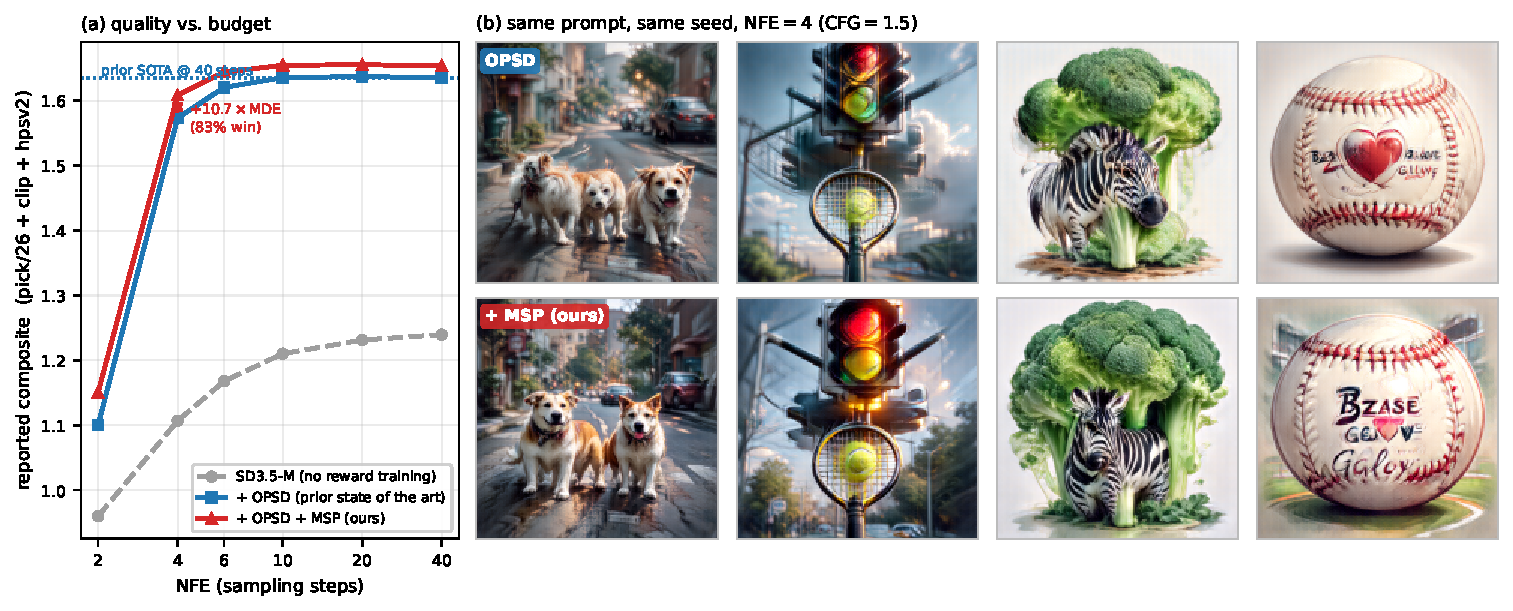
\includegraphics[width=\linewidth]{fig0_teaser.pdf}
\caption{\textbf{Multi-state target propagation (\MSP) makes on-policy reward distillation
budget-robust.} (a) Reported composite versus sampling budget on DrawBench. The prior state
of the art, \opsd, loses most of its advantage once the budget falls below $10$ steps;
propagating the \emph{same} reward-constructed target to higher-noise states of the same
rollout recovers it: on the measured grid it reaches \opsd's $40$-step quality at $6$
sampling steps, where \opsd itself needs $10$.
(b) Same prompts, same seed, $4$ sampling steps, rendered at guidance $1.5$
(App.~\ref{app:protocol}). The four prompts are drawn from the twelve selected in advance by
the rule in App.~\ref{app:qual}, which favours differences checkable by eye -- object counts,
spatial relations and text; all twelve are shown in Fig.~\ref{fig:qual}.}
\label{fig:teaser}
\end{figure}

Aligning a text-to-image diffusion model to a differentiable reward can be cast as
\emph{on-policy self-distillation}: a frozen behavior policy rolls out trajectories, a
reward gradient is converted into a detached target for an intermediate prediction, and
the trainable policy regresses onto that target~\citep{opsd2026,danceopd2026,diffusionopd2026}.
This interface is attractive because the reward and the decoder appear only during target
construction; the fitting step is an ordinary regression and does not retain the reward
graph.

Every method in this family must answer a question that, to our knowledge, has never been
studied: \textbf{at which noise level should the target be built and the loss applied?}
The strongest current method, \opsd, selects a single \emph{low-noise} query
($\sigma^\star\!=\!0.278$, the second-to-last non-degenerate state of a $10$-step
schedule) and applies its loss only there. The choice is defensible -- we confirm in
Sec.~\ref{sec:analysis} that this is where a unit of target displacement buys the most
reward -- but it is made with a single sampling budget in mind.

The consequence shows up as a gap between what a reward-distilled model produces at its
training budget and at a short one, and that gap is \emph{not} a symptom of undertraining.
Trained to the published $300$ updates rather than $100$, the canonical procedure's
$40$-step-versus-$4$-step gap \emph{widens} --- from $19.1$ to $22.3$ MDE on DrawBench and
from $17.1$ to $22.7$ on the held-out prompt set --- because extra budget improves the
full-budget sample faster than the short one. Propagating the target, at the same $100$
updates, moves the gap the other way, to $13.7$ and $12.4$. Training longer aggravates the
problem; changing where the target is applied is what relieves it.

\paragraph{This paper.} We treat the placement of the reward target as the object of
study and evaluate three answers under a strictly matched protocol
(same optimizer budget, same hardware, same seeds, per-image paired tests):

\begin{enumerate}[leftmargin=1.6em,itemsep=2pt]
\item[\textbf{(A)}] \textbf{Move the query state.} Raise $\sigma^\star$ from $0.278$ to
$0.465$. This is a one-line configuration change with \emph{zero} additional cost.
\item[\textbf{(B)}] \textbf{Shorten the training rollout} from $10$ to $6$ steps. This is
\emph{cheaper} than the baseline ($0.90\times$) and moves the query state implicitly,
because the query is selected by nearest-$\sigma$ on the schedule.
\item[\textbf{(C)}] \textbf{Propagate the target (ours).} Keep the low-noise query where
it is, and additionally use the \emph{same} detached target as the regression target at
two higher-noise states of the same rollout. This costs $1.21\times$ and, crucially,
requires \emph{no} additional reward evaluation and \emph{no} additional decoding.
\end{enumerate}

\paragraph{Findings.} (i) (A) and (B) are the same mechanism. Their gain-versus-budget
curves coincide to within measurement error on both prompt sets, and both are a
\emph{trade}: $+12.7$ and $+12.3$ MDE at $4$ sampling steps, but $-0.3$ and $-0.1$ MDE at
the full $40$-step budget ($-1.1$ and $-1.0$ on the held-out prompt set). Raising the
query noise level buys few-step quality by giving up full-budget quality.
(ii) Propagation (C) is \emph{not} a trade. It is the only one of the three
interventions that clears our significance threshold in \emph{all four}
prompt-set~$\times$~budget cells. At $40$ steps it still retains $37\%$ of its peak gain on
DrawBench and $20\%$ on the held-out set, whereas (A) and (B) retain nothing at all --
their full-budget gain has gone slightly negative.
(iii) The two compose: (B$+$C) removes (B)'s full-budget loss \emph{and} attains the
largest few-step gains in the study ($+16.23$ and $+15.91$ MDE, win rates $92.7\%$ and
$95.4\%$). Propagation therefore yields a small family of operating points from one
mechanism -- pure (C) when a single model must serve every budget, (B$+$C) when the
deployment budget is a handful of steps.

\paragraph{Contributions.}
\begin{itemize}[leftmargin=1.4em,itemsep=2pt]
\item We identify target \emph{placement} as an unexamined design axis of on-policy reward
distillation, and show that the placement used by the current state of the art is
suboptimal for few-step sampling by a large margin at zero cost (Sec.~\ref{sec:exp:where}).
\item We propose \textbf{multi-state target propagation} (\MSP): reuse one reward-constructed
target as the regression target at several noise levels of the same trajectory. \MSP adds
no reward evaluations and no decodes, and we show that its per-state backward is
mathematically identical to a joint backward while keeping peak memory at the
single-state level (Sec.~\ref{sec:method}).
\item We give a mechanistic account of why moving the query is a trade and propagating is
not, supported by a measured reward-per-displacement exchange rate across noise levels and
by the height each configuration reaches on the training objective itself
(Sec.~\ref{sec:analysis}).
\item We characterise the design space the method opens. The noise level the supervision
set reaches has an \emph{interior} optimum -- stopping lower or reaching higher are both
worse in every cell -- and the gain survives stacking on the strongest baseline in our
study, which rules out the reading that propagation only helps an under-tuned run
(App.~\ref{app:family}, \ref{app:stack}).
\item We \textbf{map the operating range} of the method rather than only its best point.
Three experiments bound it: raising the branch coefficient from the published $0.1$ to
$1.0$ reverses the gain ($+10.70\to-15.40$ MDE at four steps); training to $300$ updates
instead of $100$ removes the forty-step gain in both of two seeds, and in one of them
collapses the four-step gain as well; and the
reward-specific recipes disagree among themselves, from a significant loss to a significant
gain. We report these because they were
pre-registered comparisons, and they delimit where the method applies
(Sec.~\ref{sec:conclusion}, App.~\ref{app:rewardspec}).
\item We build on a reproduction that we verify against the published protocol rather than
assume. At the published $300$-update budget our canonical run matches the reported row on
\emph{all five} evaluators, and the untrained base model matches to within $1.6\%$, which
isolates the evaluation pipeline from any training code
(Sec.~\ref{sec:exp:repro}). We then report all results against a \emph{measured}
canonical-versus-canonical noise floor and a calibrated held-out evaluator, and release the
calibration (App.~\ref{app:floor}, \ref{app:evalcal}). We believe this protocol is of independent use
to the reward-alignment literature, where effect sizes are frequently of the same order as
run-to-run variation.
\end{itemize}

\section{Related Work}
\label{sec:related}

\paragraph{Reward-to-target interfaces.} Differentiable-reward fine-tuning of diffusion
models backpropagates a reward through the decoder into the
sampler~\citep{refl2023,draft2023}. \opsd~\citep{opsd2026} instead converts the reward
gradient into a \emph{detached} target for an intermediate clean-output prediction and
fits it as a regression, which removes the reward graph from the fitting step. Our work
takes that interface as given and studies a design choice inside it -- where the target is
placed -- rather than replacing the interface.

\paragraph{On-policy distillation.} DanceOPD~\citep{danceopd2026},
DiffusionOPD~\citep{diffusionopd2026} and FlowOPD~\citep{flowopd2026} match a frozen
teacher field at states drawn from the current policy. \MSP shares their fitting interface
but not their supervision: the target is constructed from a reward, once, and then reused
across states of the same trajectory.

\paragraph{Few-step sampling.} A separate line of work distills a diffusion model into a
few-step sampler directly (consistency and distribution-matching
objectives~\citep{lcm2023,dmd2024}, adversarial few-step
models~\citep{sdxlturbo2023}). \textbf{We do not compete with these methods and do not
claim a state-of-the-art few-step generator.} Our claim is internal to reward
distillation: given that one is running an on-policy reward-distillation procedure, the
placement of the reward target materially changes how the resulting model behaves under a
reduced sampling budget, and one placement strategy improves both regimes at once. The two
lines are orthogonal and, in principle, composable; we leave that combination to future
work.

\paragraph{Effect-size calibration.} Reported gains in reward alignment are often of the
same order as seed-to-seed variation. We follow the practice of measuring the null
directly~\citep{bouthillier2021accounting} by evaluating many unmodified baselines against
one another, and we calibrate which held-out evaluator actually tracks the training
objective before using it. Both are described in the appendix.

\section{Preliminaries}
\label{sec:prelim}

We follow the notation of \opsd~\citep{opsd2026}. Let $v_\theta$ be the trainable
rectified-flow velocity field and $v_{\mathrm{old}}$ the frozen behavior policy of the
current outer iteration. For a prompt $\vc$, a noisy latent $z_\sigma$ and a noise level
$\sigma$, write the query tuple $s=(\vc,z_\sigma,\sigma)$. Under the rectified-flow path
$z_\sigma=(1-\sigma)y+\sigma\epsilon$ the velocity target is $v=\epsilon-y$, so the
\emph{clean-output prediction} at that query is
\begin{equation}
y_\theta(s)=z_\sigma-\sigma\,v_\theta(s),
\label{eq:clean}
\end{equation}
which is decoder-evaluable through the local reward
$\widetilde R(y,\vc)=R(D(y),\vc)$.

\paragraph{Query state and anchor.} The behavior policy rolls out a trajectory with the
sampler's schedule $\{\sigma_j\}_{j=0}^{N}$. Given a \emph{requested} query level
$\sigma^\star$, the implementation selects the schedule index by nearest value,
\begin{equation}
q=\argmin_j\,|\sigma_j-\sigma^\star|,
\qquad
s_q=(\vc,z_q,\sigma_q),
\qquad
y_0=z_q-\sigma_q\,v_{\mathrm{old}}(s_q).
\label{eq:query}
\end{equation}
Both $z_q$ and $y_0$ are detached. \opsd uses $\sigma^\star=0.278$; on the $10$-step
schedule of SD3.5-Medium this selects $\sigma_q=0.27805$, the second-to-last
non-degenerate state.

\paragraph{Target construction.} Starting from $y_0$, normalized reward-gradient steps
with step size $h=\eta\rho\|y_0\|_2/M$ produce positive and negative targets, each
projected back onto the trust region $\|y_\pm-y_0\|_2\le\rho\|y_0\|_2$, and finally
detached:
\begin{equation}
\bar y_\pm=\sg\big(y_\pm^{(M)}\big),\qquad
\|\bar y_\pm-y_0\|_2\le\rho\|y_0\|_2 .
\label{eq:targets}
\end{equation}
This is the only place where the reward and the decoder are differentiated.

\paragraph{Finite fitting.} The trainable field is evaluated \emph{at the same query},
$y_\theta=z_q-\sigma_q v_\theta(s_q)$, and split into two implicit branches
$y_\theta^{+}=\beta y_\theta+(1-\beta)y_0$ and
$y_\theta^{-}=(1+\beta)y_0-\beta y_\theta$. With detached adaptive normalizers
$\gamma_\pm$ and a group-normalized weight $\omega\in[0,1]$,
\begin{equation}
\mathcal L_{\mathrm{OPSD}}(s_q;\bar y_+,\bar y_-)
=\omega\,\frac{\operatorname{mean}\big[(y_\theta^{+}-\bar y_+)^2\big]}{\gamma_+}
+(1-\omega)\,\frac{\operatorname{mean}\big[(y_\theta^{-}-\bar y_-)^2\big]}{\gamma_-}.
\label{eq:opsdloss}
\end{equation}

\paragraph{The unexamined choice.} Equations~\eqref{eq:query}--\eqref{eq:opsdloss} fix
\emph{one} state: the target is built at $s_q$ and the loss is applied at $s_q$. Nothing
in the derivation requires these to be the same state, nor that there be only one. The
rest of this paper studies what happens when that assumption is relaxed.

\section{Multi-State Target Propagation}
\label{sec:method}

\begin{figure}[t]
\centering
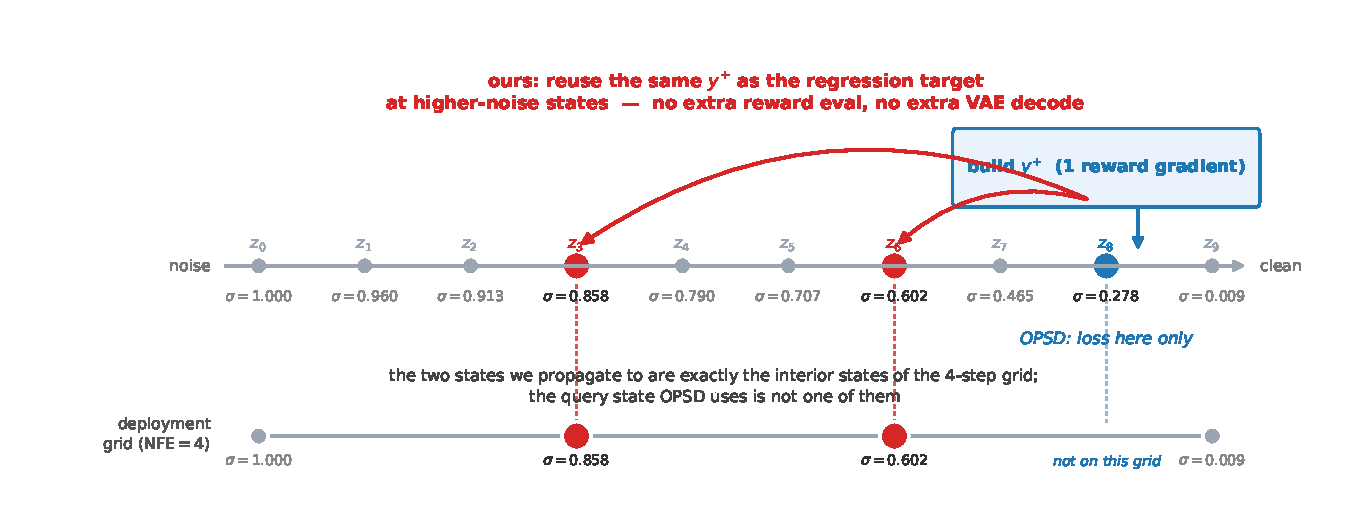
\includegraphics[width=\linewidth]{fig1_method.pdf}
\caption{\textbf{Where the reward target is applied.} The behavior policy produces a
rollout with schedule $\{\sigma_j\}$ (values shown are the actual SD3.5-M $10$-step
schedule). \opsd builds the detached target $\bar y_\pm$ at $z_8$ ($\sigma\!=\!0.278$) with
one reward gradient and applies its loss only there. \MSP reuses the \emph{same} target as
the regression target at $z_3$ and $z_6$ ($\sigma\!=\!0.858,\,0.602$), which requires no
further reward evaluation and no further decoding. The lower axis shows why those two
states: they are exactly the interior states of the four-step sampling grid
$\{1.000,\,0.858,\,0.602,\,0.009\}$, the grid the deployed model actually walks. \opsd's
query state is not on that grid at all, which is the sense in which its placement is tuned
for a different budget than the one a few-step deployment uses.}
\label{fig:method}
\end{figure}

\subsection{The target is type-correct at every noise level}

Equation~\eqref{eq:clean} defines a clean-output prediction \emph{for every query with
$\sigma>0$}, not only for the query at which the target was constructed. The detached
targets $\bar y_\pm$ of Eq.~\eqref{eq:targets} are points in that same clean-output space:
they are an estimate of a clean image, obtained by moving $y_0$ a bounded distance along
the reward gradient. Consequently, for any other state $z_k$ of the same rollout,
\begin{equation}
y_\theta(s_k)=z_k-\sigma_k v_\theta(s_k),\qquad s_k=(\vc,z_k,\sigma_k),
\end{equation}
is a quantity of the same type as $\bar y_\pm$, and regressing it onto $\bar y_\pm$ is
well-posed. This is the entire observation behind \MSP: \emph{a target built once can be
supervised many times}.

Two remarks delimit the claim. First, $\bar y_\pm$ is a target for the \emph{conditional
mean} at each state, not a claim that a single sample is reachable from $z_k$; this is
exactly the regression semantics that diffusion training already uses. Second, the
construction remains on-policy: all $z_k$ come from the same frozen-behavior-policy
trajectory that produced $z_q$.

\subsection{Objective}

Let $\mathcal K\subset\{1,\dots,N-1\}$, $q\notin\mathcal K$, be a set of additional states
of the same trajectory. \MSP replaces Eq.~\eqref{eq:opsdloss} by the uniform average
\begin{equation}
\boxed{\;
\mathcal L_{\MSP}
=\frac{1}{1+|\mathcal K|}
\Big[\;\mathcal L_{\mathrm{OPSD}}(s_q;\bar y_+,\bar y_-)
\;+\!\!\sum_{k\in\mathcal K}\!\mathcal L_{\mathrm{OPSD}}(s_k;\bar y_+,\bar y_-)\Big] \; }
\label{eq:msploss}
\end{equation}
where every term uses the \emph{same} $\bar y_\pm$, the same group weight $\omega$, and
its own adaptive normalizers $\gamma_\pm^{(k)}$ and branch anchor
$y_0^{(k)}=z_k-\sigma_k v_{\mathrm{old}}(s_k)$. The $1/(1+|\mathcal K|)$ factor keeps the
overall gradient scale comparable to the baseline; Sec.~\ref{sec:analysis} shows that this
down-weighting of the main term is not what drives the effect.

Throughout, our default is $\mathcal K=\{3,6\}$, i.e.\ $\sigma=0.858$ and $0.602$. These
are not tuned values. They are the two interior states of the $4$-step sampling grid
$\sigma\in\{1.000,\,0.858,\,0.602,\,0.009\}$ expressed on the $10$-step training grid
(all schedules are read from the model's own scheduler and listed in
App.~\ref{app:schedule}), and
we picked them for that reason; note that the canonical query $\sigma^\star\!=\!0.278$ lies
on neither grid, so \opsd supervises a state a $4$-step sampler never visits. What the data supports is
an \emph{interior optimum} in the noise level the set reaches. Replacing $\{3,6\}$ by the
lower, denser $\{5,6,7\}$ ($\sigma$ up to $0.707$) costs $2$--$3.5$ MDE at every budget from
$4$ to $40$ steps despite using \emph{more} states; replacing it by the \emph{higher}
$\{2,3,4\}$ ($\sigma$ up to $0.913$) is no better and is worse at the full budget
(App.~\ref{app:family}). The default sits between them. This matches the measured
reward-per-displacement exchange rate, which collapses from $0.457$ at $\sigma=0.278$ to
$0.007$ at $\sigma=0.913$ (Sec.~\ref{sec:analysis}): too little noise and the supervision
misses the states a few-step sampler visits, too much and the reward gradient has almost
no leverage there. Grid alignment alone does not explain the effect: among the budgets whose sampling grid has
an interior state at all, the advantage of $\{3,6\}$ over the lower set is \emph{smallest}
at exactly the budget it matches ($+2.2$ MDE at four steps, rising to $+3.5$ at twenty). At
two steps the grid has no interior state, and there the lower set is ahead by $4.8$ MDE
(App.~\ref{app:family}).

\subsection{Per-state backward is exact and memory-neutral}

Equation~\eqref{eq:msploss} is a sum of terms that share no intermediate activations:
each $\mathcal L_{\mathrm{OPSD}}(s_k;\cdot)$ requires its own forward pass of $v_\theta$
at $z_k$. Materializing all $1+|\mathcal K|$ graphs before a single backward would multiply
peak activation memory, which is prohibitive (the baseline already occupies
$79.2$ of $79.25$\,GiB on an A100). Because $\nabla_\theta$ is linear over the sum, we may
instead call backward once per state and let the gradients accumulate in
\texttt{.grad}:
\begin{equation}
\nabla_\theta\mathcal L_{\MSP}
=\frac{1}{1+|\mathcal K|}\Big[\nabla_\theta\mathcal L_{\mathrm{OPSD}}(s_q)
+\sum_{k\in\mathcal K}\nabla_\theta\mathcal L_{\mathrm{OPSD}}(s_k)\Big],
\end{equation}
which is \emph{exactly} the joint gradient while holding peak memory at the single-state
level. This is what makes the method practical rather than merely definable.

\subsection{Cost}

Each additional state costs two transformer forwards (behavior and trainable policy) and
one backward. It costs \emph{no} reward-model evaluation and \emph{no} VAE decode -- the
two dominant terms of target construction, which are incurred once regardless of
$|\mathcal K|$. Measured end-to-end over a full $100$-update run on identical hardware
(App.~\ref{app:cost}), $|\mathcal K|=2$ costs $1.21\times$ the baseline and
$|\mathcal K|=3$ costs $1.28\times$, i.e.\ $\approx\!+0.09$ to $+0.10\times$ per state.

\section{Experiments}
\label{sec:exp}

\subsection{Protocol}
\label{sec:exp:protocol}

\paragraph{Setup.} All arms fine-tune SD3.5-Medium with LoRA under an identical
$100$-optimizer-update budget, the same composite reward
($\textsc{PickScore}+\textsc{CLIP}+\textsc{HPSv2}$ on raw scores), the same data
($1152$ samples/epoch from Pick-a-Pic), $512^2$ resolution and guidance scale $1.0$.
An arm and its baseline always share \emph{training hardware, world size, random seed, and
outer epoch}; we verified that mismatching any of these produces artifacts of the same
order as the effects we report (App.~\ref{app:pairing}).

\paragraph{Evaluation.} We report the composite $\textsc{Pick}/26+\textsc{CLIP}+\textsc{HPSv2}$
on two prompt sets -- DrawBench ($200$ unique prompts $\times5$ images) and
\emph{Unseen-1k} ($1000$ unique held-out Pick-a-Pic prompts) -- generated with the
rectified-flow sampler at $\mathrm{NFE}\in\{2,4,6,10,20,40\}$, always on A40 GPUs, with
$n\!=\!1000$ images per cell. Differences are per-image paired and reported in units of
$\mathrm{MDE}=0.0033$.

\paragraph{What counts as an effect.} Effect sizes in this literature are often comparable
to run-to-run variation, so we measured the variation directly: across $8$ unmodified
canonical arms (differing only in hardware, world size or seed) the $28$ pairwise
differences have median $|\Delta|=0.39$ MDE and maximum $1.23$ MDE; two runs of the
\emph{identical} configuration differ by $0.56$ MDE (App.~\ref{app:floor}). We therefore
require $|\Delta|\ge2.5$ MDE with $t>2$ for a single-seed claim, or $1$--$2.5$ MDE with a
same-signed second seed.

\paragraph{Held-out evaluator.} Across $12$ arms spanning $-35$ to $+18$ MDE, ImageReward
tracks the reported composite ($r=+0.894$, sign agreement $12/12$) whereas Aesthetic is
\emph{anti}-correlated ($r=-0.395$, $4/12$). We therefore report ImageReward as the
held-out evaluator and do not report Aesthetic (App.~\ref{app:evalcal}).

\subsection{Reproduction fidelity}
\label{sec:exp:repro}

Before any comparison we check that our reproduction and our evaluation agree with the
published protocol. We match it on every axis we could verify: LoRA rank $32$ and alpha
$64$ at $512^2$, Pick-a-Pic training prompts, CFG-free rollouts with guidance $1.0$ and a
deterministic $10$-step DPM-Solver++ 2M, $48$ prompt groups of $24$ images per optimizer
update, AdamW at $3\times10^{-4}$, trust region $\rho=0.10$, two target steps,
branch coefficient $\beta=0.1$ for the joint three-reward objective and $1.0$ for
reward-specific runs, checkpoint-averaged parameters at save time, and DrawBench
evaluation with $40$-step flow sampling at guidance $1.0$.

Table~\ref{tab:official} puts the two side by side. The untrained base model -- which
involves no training code at all, and therefore isolates the evaluation pipeline -- agrees
with the published numbers to $0.4\%$ on PickScore, $1.6\%$ on CLIPScore, $1.5\%$ on
HPSv2.1 and $0.1\%$ on Aesthetic. That row is marked in the source as partly inherited from
an earlier report rather than re-measured, so we treat it as a check on the protocol rather
than on any one group's measurement.

\paragraph{The joint objective at the published budget.} Trained for the published $300$
updates, our reproduction lands within the measurement tolerance on \emph{all five}
evaluators:

\begin{center}
\begin{tabular}{lccccc}
\toprule
& Pick & CLIP & HPSv2.1 & Aes & ImgR\\
\midrule
reported \citep{opsd2026} & $25.51$ & $0.333$ & $0.389$ & $6.03$ & $1.51$\\
ours, $300$ updates       & $25.46$ & $0.332$ & $0.388$ & $5.95$ & $1.51$\\
\midrule
$|\Delta|$ as a fraction of tolerance & $0.12$ & $0.21$ & $0.19$ & $0.81$ & $0.11$\\
\bottomrule
\end{tabular}
\end{center}

The tolerance is not chosen after the fact: it is the $1.6\%$ agreement measured on the
untrained backbone above, which bounds what the evaluation pipeline alone can account for,
and seven unmodified canonical runs spanning three GPU types, two world sizes and two seeds
vary by at most $0.65$ of that tolerance on any column (App.~\ref{app:floor}). Our numbers
are consistently a touch below the published ones, but the largest gap is $0.81$ of the
tolerance and the median is $0.19$, so the offset is not separable from the pipeline itself.
We therefore read the published method as reproduced at its own budget, and report the
baselines it is compared against as inherited rather than re-measured.

Table~\ref{tab:official} also carries the baselines reported alongside \opsd. We did not
rerun them; the upper block is reproduced from that paper so that our numbers can be read
against the same field, and we mark it as such rather than presenting it as our
measurement. One entry is worth noting even at this stage: at $100$ updates \MSP already
reaches the ImageReward value that \opsd reports at $300$ ($1.51$), and exceeds every
non-\opsd baseline in that column, including DiffusionNFT at $300$ updates ($1.45$) and
FlowGRPO at $4$k ($1.29$). That value also matches our \emph{own} canonical run at the
full $300$ updates ($1.5066$), so the comparison does not depend on reading across
laboratories. \MSP at $100$ updates remains below the $300$-update row on the three
components of the training composite, which is what a third of the budget should give, so
this is an observation about the held-out column and not a claim that a third of the budget
suffices; the matched $300$-update \MSP run is still training.

The stronger check is a \emph{trained} checkpoint, and here the published numbers are ones
the original authors measured themselves rather than inherited. The reward-specific block is
trained under a different recipe from the joint one --- $100$ updates and $\beta=1.0$ rather
than $300$ and $0.1$ --- so it is an independent test of the same code. Reproducing it gives
HPSv2.1 $0.3920$ against a reported $0.390$ ($0.5\%$) and PickScore $24.96$ against $24.94$
($0.08\%$). The CLIPScore column is the one place our reproduction falls outside that
tolerance: $0.3203$ against a reported $0.340$, a gap of $5.9\%$. The evaluator is not the
cause --- our CLIPScore agrees with the published value to $1.6\%$ on the untrained backbone
and to $0.33\%$ on the joint $300$-update row --- so the gap is specific to the
CLIPScore-trained run, which is still improving when its budget ends. We report it rather
than tune towards it (App.~\ref{app:rewardspec}); the two remaining columns are not yet
available.
Those numbers exercise the training code, the target construction and the evaluation
together, and their deviations run in the opposite direction from the joint block's, so
there is no systematic offset. We take the reproduction as verified rather than assumed.

We also checked that one published hyper-parameter is not arbitrary. The protocol sets the
branch coefficient to $\beta=0.1$ for the joint objective; retraining the canonical arm at
$\beta=1.0$ and changing nothing else costs it $5.09$ and $6.09$ MDE on DrawBench at $4$ and
$40$ steps, and $5.45$ and $6.02$ on the held-out prompt set, with per-image win rates of
$20$--$27\%$. The published value is therefore tightly tuned for this objective. (That arm
ran on a different accelerator from its control; the offset such a swap induces is
$\le0.55$ MDE, App.~\ref{app:pairing}, against an effect of $5$--$6$.)

% 自动生成,勿手改。源:paper_figs/make_table_official.py
\begin{table}[t]
\centering
\setlength{\tabcolsep}{4pt}
\caption{\textbf{SD3.5-M under the published protocol.} DrawBench, $40$-step flow,
guidance $1.0$, $512^2$, $n{=}1000$, checkpoint-averaged parameters. The upper block is
reproduced verbatim from \citet{opsd2026}; we did not rerun those baselines. The lower
block is ours under the same protocol. \cmark: one checkpoint per evaluator column;
\xmark: a single checkpoint evaluated across all columns. Higher is better.}
\label{tab:official}
\resizebox{0.98\linewidth}{!}{%
\begin{tabular}{lcc rrrrr}
\toprule
\textbf{Model} & \textbf{R.-spec.} & \textbf{Upd.} & \textbf{Pick} & \textbf{CLIP} & \textbf{HPSv2.1} & \textbf{Aes} & \textbf{ImgR}\\
\midrule
\multicolumn{8}{l}{\textbf{Reported by \citet{opsd2026}}}\\
\midrule
\multicolumn{8}{l}{\emph{Reference backbones}}\\
\quad SDXL & \xmark & -- & $22.42$ & $0.287$ & $0.280$ & $5.60$ & $0.76$\\
\quad SD3.5-L & \xmark & -- & $22.91$ & $0.289$ & $0.288$ & $5.50$ & $0.96$\\
\quad FLUX.1-dev & \xmark & -- & $22.84$ & $0.295$ & $0.274$ & $5.71$ & $0.96$\\
\midrule
\multicolumn{8}{l}{\emph{SD3.5-M, one checkpoint across all columns}}\\
\quad SD3.5-M w/o CFG & \xmark & -- & $20.51$ & $0.237$ & $0.204$ & $5.13$ & $-0.58$\\
\quad $+$ CFG & \xmark & -- & $22.34$ & $0.285$ & $0.279$ & $5.36$ & $0.85$\\
\quad $+$ FlowGRPO & \xmark & 4k & $23.50$ & $0.280$ & $0.316$ & $5.90$ & $1.29$\\
\quad $+$ DiffusionNFT & \xmark & 300 & $23.62$ & $0.294$ & $0.340$ & $6.02$ & $1.45$\\
\quad $+$ DanceOPD & \xmark & 300 & $23.06$ & $0.272$ & $0.322$ & $5.98$ & $1.23$\\
\quad $+$ DiffusionOPD & \xmark & 300 & $23.05$ & $0.269$ & $0.322$ & $6.04$ & $1.23$\\
\quad $+$ FlowOPD & \xmark & 300 & $22.62$ & $0.263$ & $0.300$ & $5.98$ & $0.92$\\
\quad $+$ \opsd & \xmark & 300 & $25.51$ & $0.333$ & $0.389$ & $6.03$ & $1.51$\\
\midrule
\multicolumn{8}{l}{\emph{SD3.5-M, one checkpoint per evaluator}}\\
\quad $+$ ReFL & \cmark & 100 & $23.92$ & $0.308$ & $0.358$ & $12.09$ & $1.28$\\
\quad $+$ DiffusionNFT & \cmark & 100 & $23.43$ & $0.298$ & $0.336$ & $9.11$ & $1.46$\\
\quad $+$ \opsd & \cmark & 100 & $24.94$ & $0.340$ & $0.390$ & $12.08$ & $1.76$\\
\midrule
\multicolumn{8}{l}{\textbf{Ours, same protocol}}\\
\midrule
\quad SD3.5-M w/o CFG & \xmark & -- & $20.59$ & $0.241$ & $0.207$ & $5.12$ & $-0.55$\\
\quad $+$ \opsd (repro) & \xmark & 100 & $24.66$ & $0.316$ & $0.370$ & $5.90$ & $1.43$\\
\quad $+$ \opsd (repro) & \xmark & 300 & $25.46$ & $0.332$ & $0.388$ & $5.95$ & $1.51$\\
\quad $+$ \MSP (ours) & \xmark & 100 & $24.84$ & $0.323$ & $0.376$ & $5.94$ & $1.51$\\
\quad $+$ \MSP (ours) & \xmark & 300 & $25.11$ & $0.327$ & $0.376$ & $5.94$ & $1.41$\\
\midrule
\multicolumn{8}{l}{\emph{SD3.5-M, one checkpoint per evaluator}}\\
\quad $+$ \opsd (repro) & \cmark & 100 & $24.96$ & $0.320$ & $0.392$ & $12.18$ & $1.76$\\
\quad $+$ \MSP (ours) & \cmark & 100 & $24.95$ & $0.319$ & $0.391$ & $9.47$ & $1.79$\\
\bottomrule
\end{tabular}}
\end{table}


\subsection{Main results}
\label{sec:exp:main}

% 主表 — 自动生成,勿手改。源:paper_figs/make_table_main.py
\begin{table}[t]
\centering
\setlength{\tabcolsep}{3.5pt}
\caption{\textbf{Main results on DrawBench} (SD3.5-Medium, $100$ optimizer updates, A40 eval,
$n{=}1000$ prompts). Absolute scores; \textbf{bold}: best, \underline{underline}: second best.
Composite $=$ PickScore$/26+$CLIP$+$HPSv2 is the reported metric; ImageReward is the held-out
evaluator and is never trained on. Rows marked ``--'' are baselines we have not run yet.
The (A) row was trained on $3$ processes rather than $4$; the offset this induces is $0.17$ MDE
(App.~\ref{app:pairing}).}
\label{tab:main}
\resizebox{0.98\linewidth}{!}{%
\begin{tabular}{l ccccc ccccc}
\toprule
& \multicolumn{5}{c}{\textbf{NFE}$=$\textbf{4}} & \multicolumn{5}{c}{\textbf{NFE}$=$\textbf{40}} \\
\cmidrule(lr){2-6}\cmidrule(lr){7-11}
\textbf{Method} & \textbf{PickScore} & \textbf{CLIP} & \textbf{HPSv2} & \textbf{Composite} & \textbf{ImageReward} & \textbf{PickScore} & \textbf{CLIP} & \textbf{HPSv2} & \textbf{Composite} & \textbf{ImageReward} \\
\midrule
SD3.5-M (no reward training) & 19.64 & 0.2170 & 0.1343 & 1.1069 & -1.705 & 20.59 & 0.2408 & 0.2070 & 1.2396 & -0.548 \\
\quad + SFT on teacher rollouts & -- & -- & -- & -- & -- & -- & -- & -- & -- & -- \\
\quad + few-step distillation (DMD2/TDM) & -- & -- & -- & -- & -- & -- & -- & -- & -- & -- \\
\midrule
\quad + OPSD \citep{opsd2026} \emph{(prior SOTA)} & 23.97 & 0.3100 & 0.3413 & 1.5732 & 1.304 & 24.66 & 0.3165 & 0.3704 & 1.6353 & 1.433 \\
\quad\quad (A) query $\sigma$ 0.278$\to$0.465 & \underline{24.40} & 0.3189 & \underline{0.3592} & \underline{1.6166} & 1.416 & 24.67 & 0.3164 & 0.3685 & 1.6337 & 1.460 \\
\quad\quad (B) rollout 10$\to$6 & 24.39 & 0.3167 & 0.3591 & 1.6138 & 1.404 & 24.70 & 0.3149 & 0.3701 & 1.6351 & 1.458 \\
\quad\quad \textbf{(C) $+$ \MSP (ours)} & 24.26 & \underline{0.3208} & 0.3547 & 1.6085 & \underline{1.435} & \textbf{24.84} & \textbf{0.3228} & \textbf{0.3758} & \textbf{1.6538} & \textbf{1.507} \\
\quad\quad (B$+$C) & \textbf{24.53} & \textbf{0.3212} & \textbf{0.3621} & \textbf{1.6268} & \textbf{1.456} & \underline{24.77} & \underline{0.3183} & \underline{0.3717} & \underline{1.6427} & \underline{1.469} \\
\bottomrule
\end{tabular}}
\end{table}


Table~\ref{tab:main} reports absolute scores. \MSP is the best configuration at the full
budget on every axis we report -- composite $1.6538$ and held-out ImageReward $1.5072$ --
and at $4$ steps it already reaches $98.4\%$ of the composite that \opsd attains with
$40$ network evaluations ($1.6085$ vs.\ $1.6353$) -- a $10\times$ reduction in sampling
cost for a $1.6\%$ shortfall. Combining \MSP with a shortened rollout is stronger still at
$4$ steps, taking every axis in the table.

\paragraph{What is the gain worth in training budget?} Our $300$-update reproduction gives
a second reading of the same effect. Within that single run, going from $100$ to $300$
updates --- three times the training compute --- is worth $+15.92$ MDE at four steps on
DrawBench and $+16.65$ on Unseen-1k. Propagation, at $1.21\times$ the cost of a $100$-update
run, is worth $+10.70$ and $+8.20$ on the same cells:

\begin{center}
\begin{tabular}{lcccc}
\toprule
& \multicolumn{2}{c}{DrawBench} & \multicolumn{2}{c}{Unseen-1k}\\
\cmidrule(lr){2-3}\cmidrule(lr){4-5}
& NFE$=4$ & $40$ & NFE$=4$ & $40$\\
\midrule
$3\times$ the training budget ($100\!\to\!300$) & $+15.92$ & $+19.11$ & $+16.65$ & $+22.27$\\
propagation at $100$ updates & $+10.70$ & $+5.62$ & $+8.20$ & $+3.34$\\
\midrule
fraction of the budget increase & $\mathbf{67\%}$ & $29\%$ & $\mathbf{49\%}$ & $15\%$\\
per unit of extra training compute & $\mathbf{6.4\times}$ & $2.8\times$ & $\mathbf{4.7\times}$ & $1.4\times$\\
\bottomrule
\end{tabular}
\end{center}

At four steps propagation recovers half to two thirds of what tripling the budget buys,
for a tenth of the extra compute --- and the ratio is largest exactly where the method is
claimed to act. This is a statement about \emph{marginal} return from $100$ updates: \MSP at
$100$ updates does not overtake the canonical run at $300$ in absolute terms, and the
marginal value of budget is itself budget-dependent, so the conversion should not be
extrapolated beyond this range. The $1.21\times$ figure is measured on two accelerators
(App.~\ref{app:cost}), and the $100$-update checkpoint of the $300$-update run matches the
separately trained $100$-update arm to within the measured floor ($\le0.32$ MDE,
$|t|\le1.35$), so the comparison carries no cross-run confound.

\paragraph{Budget makes the problem worse, not better.} The same $300$-update run also
settles whether the few-step shortfall is simply undertraining. Measuring each model against
\emph{itself} --- its $40$-step score minus its $4$-step score --- the canonical procedure's
deficit grows monotonically with training, from $12.4$ MDE at $20$ updates to $18.8$ at
$100$ and $22.3$ at the published $300$ (DrawBench; $12.0$, $17.3$ and $22.7$ on Unseen-1k).
Extra budget improves the full-budget sample faster than the short one, so the two pull
apart. Propagation moves the curve down at every checkpoint we measured, by $2.1$ to $5.2$
MDE (Fig.~\ref{fig:deficit}). Training longer is not a substitute for changing where the
target is applied; it is what makes the change necessary.

\begin{figure}[h]
\centering
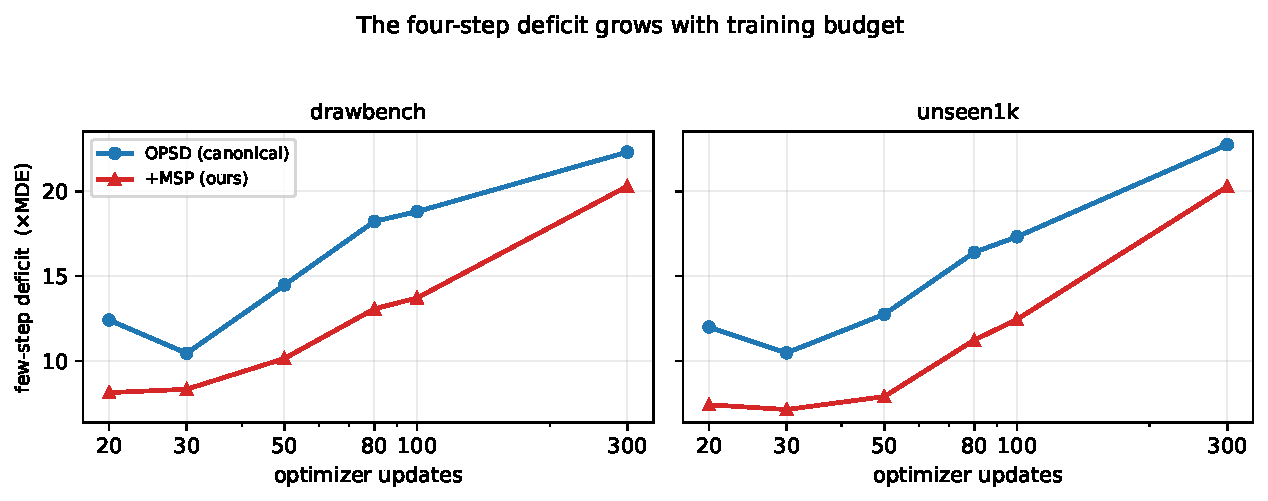
\includegraphics[width=\linewidth]{fig10_deficit_vs_budget.pdf}
\caption{\textbf{The four-step deficit grows with training budget.} Each point is one model
measured against itself: its $40$-step score minus its $4$-step score, paired over $1000$
images. Higher is worse. The canonical curve rises throughout; propagation sits below it at
every checkpoint. The dip at $30$ updates appears on both prompt sets and both arms, so it
belongs to the training trajectory rather than to evaluation noise. The $300$-update point
for propagation is still training and is omitted rather than estimated.}
\label{fig:deficit}
\end{figure}

\begin{figure}[t]
\centering
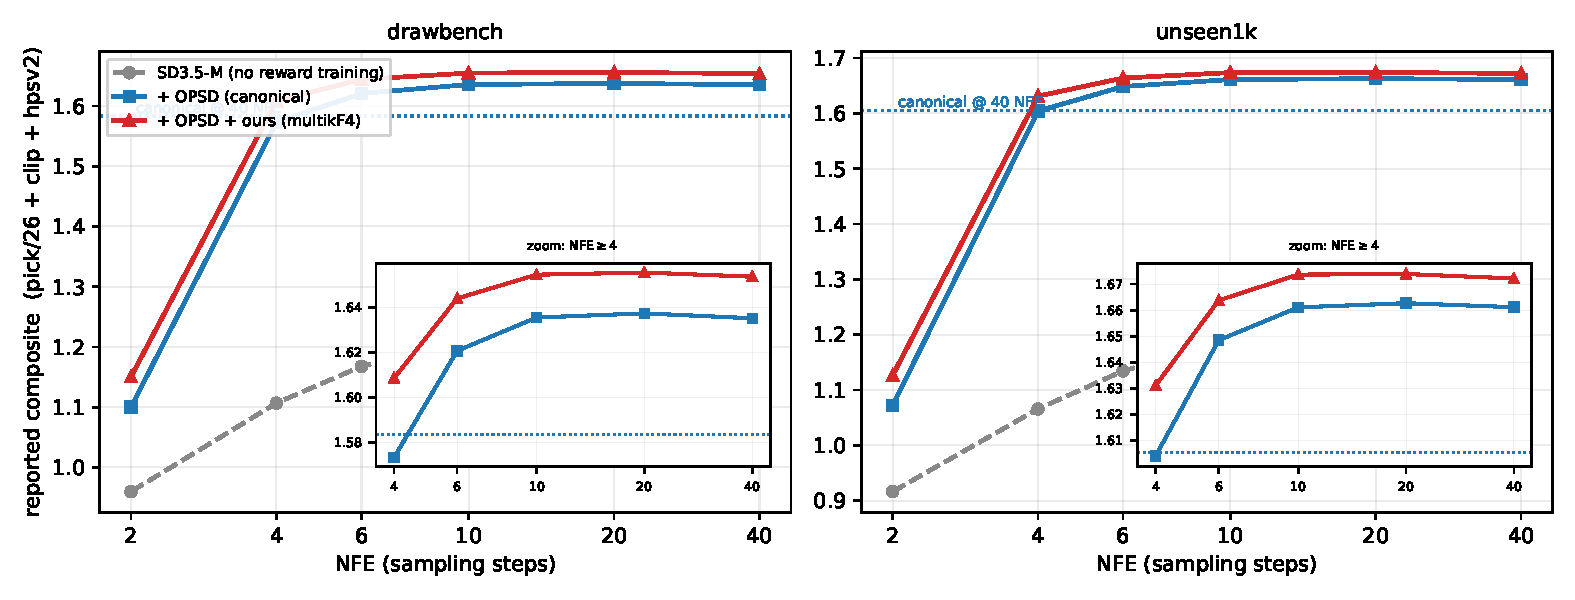
\includegraphics[width=\linewidth]{fig2_quality_vs_nfe.pdf}
\caption{\textbf{Absolute quality versus sampling budget}, both prompt sets. Dotted line:
\opsd evaluated with $40$ steps. On the measured grid \MSP crosses that line at $6$ steps
($5.4$ by interpolation); \opsd itself needs $10$.}
\label{fig:quality}
\end{figure}

\subsection{Where should the target be applied?}
\label{sec:exp:where}

% Table 1 — 自动生成,勿手改。源:paper_figs/make_table1.py
% 口径:SD3.5-M,100 optimizer updates,A40,逐图配对 n=1000/格,MDE=0.0033
\begin{table}[t]
\centering
\setlength{\tabcolsep}{4pt}
\caption{\textbf{Where should the on-policy reward target be applied?} Paired per-image gain over
the canonical OPSD model trained at the \emph{same} budget and on the \emph{same} hardware,
in units of MDE$=0.0033$; win\% in parentheses. A cell counts as a gain when it clears
$2.5\times$MDE with $t>2$, the threshold calibrated against the measured canonical-versus-canonical
noise floor (Sec.~\ref{sec:exp:protocol}); $^\dagger$ marks the $1$--$2.5\times$MDE band, which a single
seed cannot resolve. The last column counts cells that clear the threshold: propagation is the only
\emph{placement} positive at every budget on both prompt sets. The final row is a \emph{reference},
not a placement choice and not a matched-budget comparison: it is the same run read at $300$
rather than $100$ updates, included because tripling the budget is the obvious alternative. It
gains more in absolute terms, at $3.00\times$ the cost; Sec.~\ref{sec:exp:main} gives the
per-unit-compute comparison and Fig.~\ref{fig:deficit} shows that it \emph{widens} the
few-step gap that propagation narrows.}
\label{tab:where}
\resizebox{0.98\linewidth}{!}{%
\begin{tabular}{lcc cc cc c}
\toprule
& & & \multicolumn{2}{c}{\textbf{DrawBench}} & \multicolumn{2}{c}{\textbf{Unseen-1k}} & \\
\cmidrule(lr){4-5}\cmidrule(lr){6-7}
\textbf{Intervention} & \textbf{Cost} & \textbf{Setting} & NFE$=$4 & NFE$=$40 & NFE$=$4 & NFE$=$40 & \textbf{Gains} \\
\midrule
(A) move query state $\sigma$ 0.278$\to$0.465 & $1.00\times$ & \scriptsize ck100, np3 & $+12.71$ \scriptsize(89\%) & $-0.32$ \scriptsize(47\%) & $+13.18$ \scriptsize(94\%) & $-1.09$ \scriptsize(42\%) & $2/4$ \\
(B) shorten rollout 10$\to$6 steps & $0.90\times$ & \scriptsize ck100, np4 & $+12.30$ \scriptsize(91\%) & $-0.05$ \scriptsize(48\%) & $+12.43$ \scriptsize(94\%) & $-0.98$ \scriptsize(43\%) & $2/4$ \\
(C) propagate target to 2 extra states (ours) & $1.20\times$ & \scriptsize ck100, np4 & $+10.70$ \scriptsize(83\%) & $+5.62$ \scriptsize(71\%) & $+8.20$ \scriptsize(80\%) & $+3.34$ \scriptsize(64\%) & $\mathbf{4/4}$ \\
(B$+$C) rollout 6 $+$ propagation & $\sim\!1.10\times$ & \scriptsize ck100, np4 & $+16.23$ \scriptsize(93\%) & $+2.26^{\dagger}$ \scriptsize(56\%) & $+15.91$ \scriptsize(95\%) & $+1.45^{\dagger}$ \scriptsize(54\%) & $2/4$ \\
(A$+$C) query $\sigma$ 0.465 $+$ propagation & $1.20\times$ & \scriptsize ck100, np4 & $+17.00$ \scriptsize(94\%) & $+2.14^{\dagger}$ \scriptsize(57\%) & $+15.32$ \scriptsize(93\%) & $+0.70$ \scriptsize(52\%) & $2/4$ \\
\midrule
\;\emph{(reference)} train $3\times$ longer & $3.00\times$ & \scriptsize ck300 vs ck100, np4 & $+15.92$ \scriptsize(92\%) & $+19.11$ \scriptsize(95\%) & $+16.65$ \scriptsize(94\%) & $+22.27$ \scriptsize(98\%) & $\mathbf{4/4}$ \\
\bottomrule
\end{tabular}}
\end{table}


Table~\ref{tab:where} isolates \emph{where} the gain comes from. Three observations.

\textbf{(A) and (B) are the same intervention.} Moving the query state
($\sigma^\star\!:\,0.278\!\to\!0.465$) and shortening the rollout ($10\!\to\!6$ steps)
agree cell-by-cell: $+12.71$ vs.\ $+12.30$ and $+13.18$ vs.\ $+12.43$ at $4$ steps,
$-0.32$ vs.\ $-0.05$ and $-1.09$ vs.\ $-0.98$ at $40$ steps. This is expected: a $6$-step
schedule has no state near $\sigma\!=\!0.278$, so its nearest-$\sigma$ query lands at
$\sigma_q=0.432$. Shortening the rollout \emph{is} moving the query state.

\textbf{Both are a trade.} Their few-step gains are the largest single-intervention
numbers in the table, but at the full budget they are zero to significantly negative
($-1.09$, $t=-3.73$ on Unseen-1k). Raising the query noise level reallocates optimization
from low-noise refinement to mid-noise structure; few-step sampling depends more on the
latter, full-budget sampling has enough low-noise steps to do the former itself.

\textbf{Propagation is not a trade.} \MSP gains at every budget, and is the only
\emph{placement} in the table that is positive at $40$ steps on both prompt sets
($+5.62$, $+3.34$); the reference row that simply trains three times longer is also
positive there, at $3.00\times$ the cost and while widening the four-step deficit.

\begin{figure}[t]
\centering
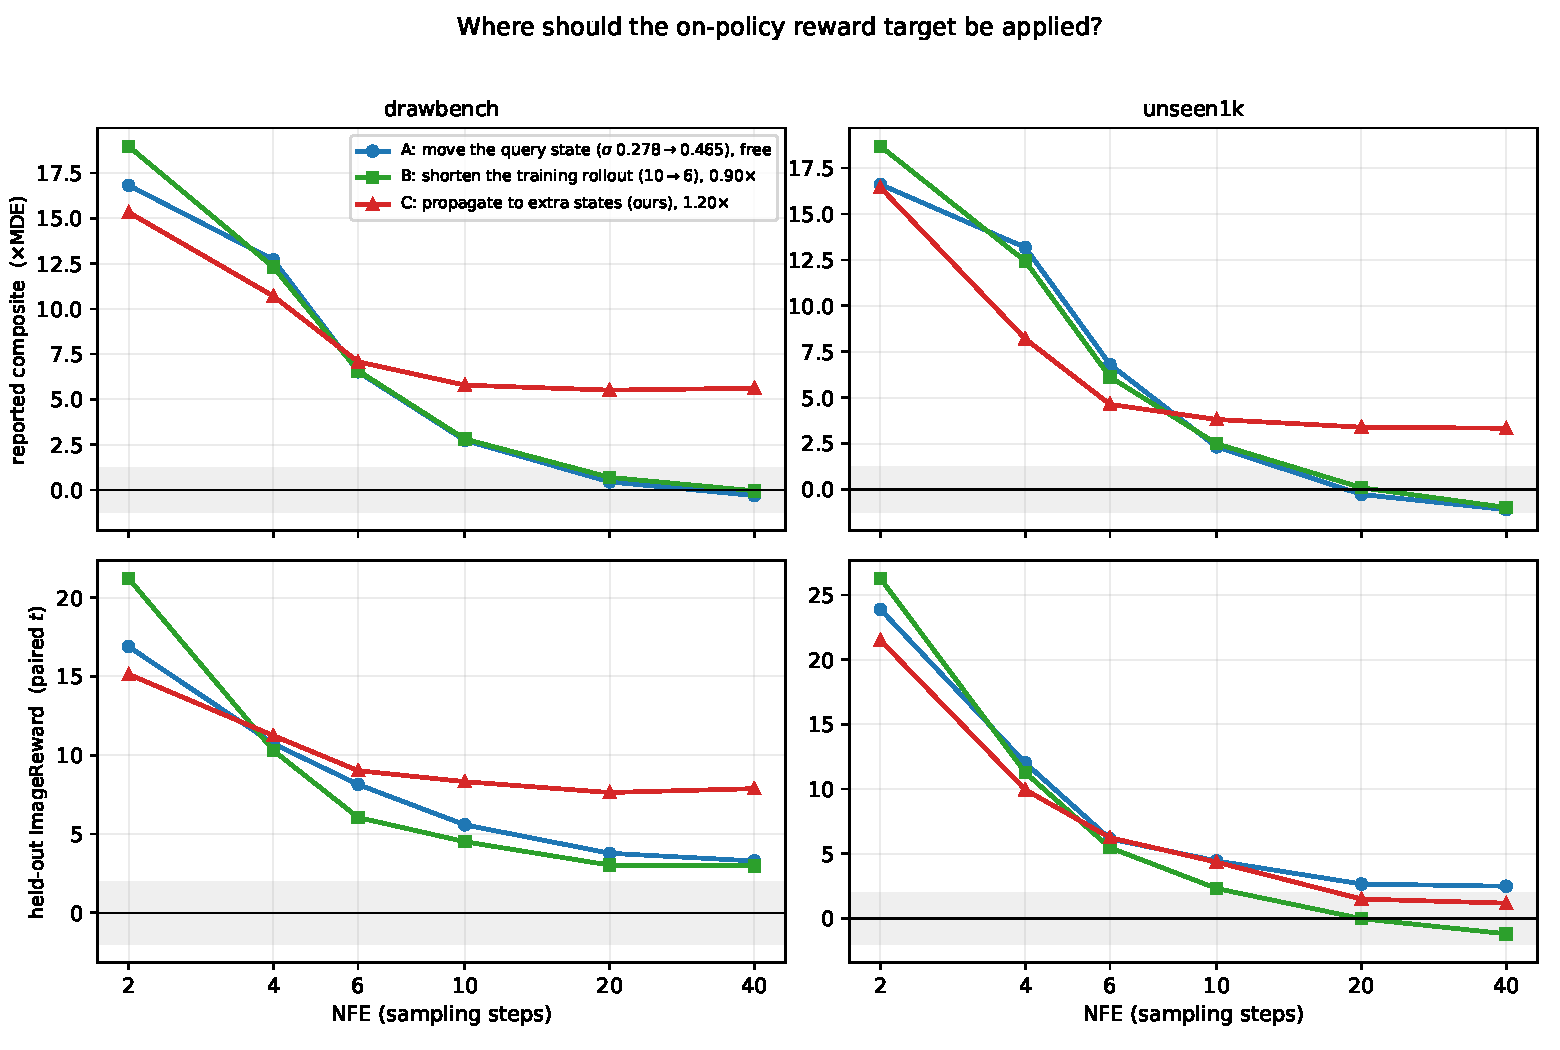
\includegraphics[width=\linewidth]{fig7_where_to_apply.pdf}
\caption{\textbf{Gain versus sampling budget.} Top: reported composite, in MDE. Bottom:
held-out ImageReward, paired $t$. Shaded band is the measured canonical-versus-canonical
floor (top) and $|t|<2$ (bottom). (A) and (B) decay to zero or below by $40$ steps;
(C) flattens at a positive value.}
\label{fig:curves}
\end{figure}

Figure~\ref{fig:curves} shows the full budget sweep. Normalizing each curve by its own
peak, \MSP retains $0.37$ of its peak gain at $40$ steps while the low-step rollout retains
$0.03$ -- the two interventions have different \emph{shapes}, not merely different sizes.

\subsection{Composition}
\label{sec:exp:compose}

% Table 3 — 自动生成。组合与增量。
\begin{table}[t]
\centering
\setlength{\tabcolsep}{4pt}
\caption{\textbf{Composition.} Propagation stacks on top of a shortened rollout.
Top block: each configuration against the canonical baseline. Bottom row: the
\emph{increment} contributed by propagation on top of the shortened rollout.
Units of MDE, win\% in parentheses; $100$ updates, matched hardware and seed.}
\label{tab:compose}
\resizebox{\linewidth}{!}{%
\begin{tabular}{lc cc cc}
\toprule
& & \multicolumn{2}{c}{\textbf{DrawBench}} & \multicolumn{2}{c}{\textbf{Unseen-1k}} \\
\cmidrule(lr){3-4}\cmidrule(lr){5-6}
\textbf{Configuration} & \textbf{Cost} & NFE$=$4 & NFE$=$40 & NFE$=$4 & NFE$=$40 \\
\midrule
(B) shortened rollout & $0.90\times$ & $+12.30$ \scriptsize(91\%) & $-0.05$ \scriptsize(48\%) & $+12.43$ \scriptsize(94\%) & $-0.98$ \scriptsize(43\%) \\
(C) \MSP & $1.20\times$ & $+10.70$ \scriptsize(83\%) & $+5.62$ \scriptsize(71\%) & $+8.20$ \scriptsize(80\%) & $+3.34$ \scriptsize(64\%) \\
\textbf{(B$+$C)} & $\sim\!1.10\times$ & $+16.23$ \scriptsize(93\%) & $+2.26$ \scriptsize(56\%) & $+15.91$ \scriptsize(95\%) & $+1.45$ \scriptsize(54\%) \\
\midrule
\quad increment of (C) over (B) & -- & $+3.93$ \scriptsize(67\%) & $+2.32$ \scriptsize(59\%) & $+3.48$ \scriptsize(70\%) & $+2.43$ \scriptsize(63\%) \\
\bottomrule
\end{tabular}}
\end{table}


\MSP composes with the cheap intervention rather than competing with it
(Table~\ref{tab:compose}). The increment contributed by propagation on top of a $6$-step
rollout is positive in all four cells -- $+3.93$ and $+2.32$ MDE on DrawBench,
$+3.48$ and $+2.43$ on Unseen-1k at $4$ and $40$ steps ($t$ from $+6.8$ to $+13.3$) -- and
it converts (B)'s full-budget loss into a gain. The resulting configuration attains the
largest few-step numbers in the study: $+16.23$ MDE ($92.7\%$ win rate) and $+15.91$ MDE
($95.4\%$). The increment grows with training (from $+3.10/+1.47$ at $50$ updates), which
is the opposite of what an under-training artifact would do.

The two configurations are complementary operating points of the same mechanism. Against
\emph{pure} \MSP, (B$+$C) trades $-3.35$ and $-1.88$ MDE at the full budget for $+5.53$ and
$+7.71$ MDE at $4$ steps -- a favourable exchange whenever inference is the bottleneck,
which is precisely the regime few-step samplers are built for. A practical reading:
\emph{if you will deploy at few steps, use (B$+$C); if one model must serve every budget,
use (C); if you can change only one line, use (A).}

\subsection{Replication and robustness}
\label{sec:exp:robust}

\paragraph{Seeds.} A second random seed, run on different hardware and at a different
world size, and compared against \emph{its own} matched canonical baseline, reproduces the
effect. At $50$ updates all four cells replicate with slightly larger magnitude --
$+8.45$ vs.\ $+7.52$ and $+4.04$ vs.\ $+3.19$ (DrawBench, $4$ and $40$ steps),
$+6.50$ vs.\ $+6.06$ and $+1.69$ vs.\ $+1.22$ (Unseen-1k) -- with a largest seed-to-seed
difference of $0.93$ MDE, below the measured floor. At $100$ updates the two DrawBench
cells give $+9.65$ and $+3.90$ against $+10.70$ and $+5.62$: the same sign, both still
clearing the threshold, with differences of $1.05$ and $1.72$ MDE. The second of those
exceeds the same-configuration floor, but these two runs differ in hardware and world size
as well as in seed, so we read it as agreement in sign and significance rather than in
magnitude.

\paragraph{Training checkpoint.} The few-step gain does not depend on where training is
stopped. A dense checkpoint sweep of the $\mathcal K=\{5,6,7\}$ family member -- the one for
which per-checkpoint canonical controls exist on matched hardware -- is positive at every
point ($20$, $30$, $50$, $80$, $100$ updates: $+8.16$, $+5.43$, $+7.05$, $+9.15$, $+8.48$
MDE on DrawBench; $+7.37$, $+5.38$, $+6.09$, $+7.62$, $+6.47$ on Unseen-1k). The default
$\mathcal K=\{3,6\}$ is measurable at five checkpoints against same-hardware controls. At
$4$ steps it clears the threshold at every one of them -- $+6.66$, $+5.56$, $+7.52$,
$+10.42$, $+10.70$ MDE on DrawBench at $20$, $30$, $50$, $80$ and $100$ updates, and
$+5.95$, $+4.83$, $+6.06$, $+8.19$, $+8.20$ on Unseen-1k -- so over this range the few-step gain
is not an artifact of extended training, and it has essentially plateaued by $80$ updates.
The \emph{full-budget} gain behaves differently across the same range: it grows
($+2.39\!\to\!+5.62$ on DrawBench, $+1.38\!\to\!+3.34$ on Unseen-1k) and only clears the
threshold on both prompt sets at $100$ updates. The two sampling budgets therefore mature at
different rates, and the claim that propagation gains at every sampling budget is one we can
make at $100$ updates, not at $20$ (App.~\ref{app:ckpt}).

\textbf{Both statements are bounded above by $100$ updates.} Trained to the published $300$
instead, the comparison reverses: propagation ends $7.2$ MDE behind at four steps and $9.2$
behind at forty on DrawBench. We report that run in Table~\ref{tab:official} and analyse it
in App.~\ref{app:ckpt}; everything claimed above is at $100$ updates, which is the budget at
which all of our comparisons are matched.

\paragraph{Per-axis.} On DrawBench all four reward axes are positive at all six budgets
and grow monotonically as the budget shrinks. On Unseen-1k the held-out ImageReward is
significant for $\mathrm{NFE}\le10$ and not significant at $20$ and $40$
($t=+1.50,+1.18$); we state this limitation rather than aggregating it away
(App.~\ref{app:peraxis}).

\subsection{Qualitative}
\label{sec:exp:qual}

\begin{figure}[t]
\centering
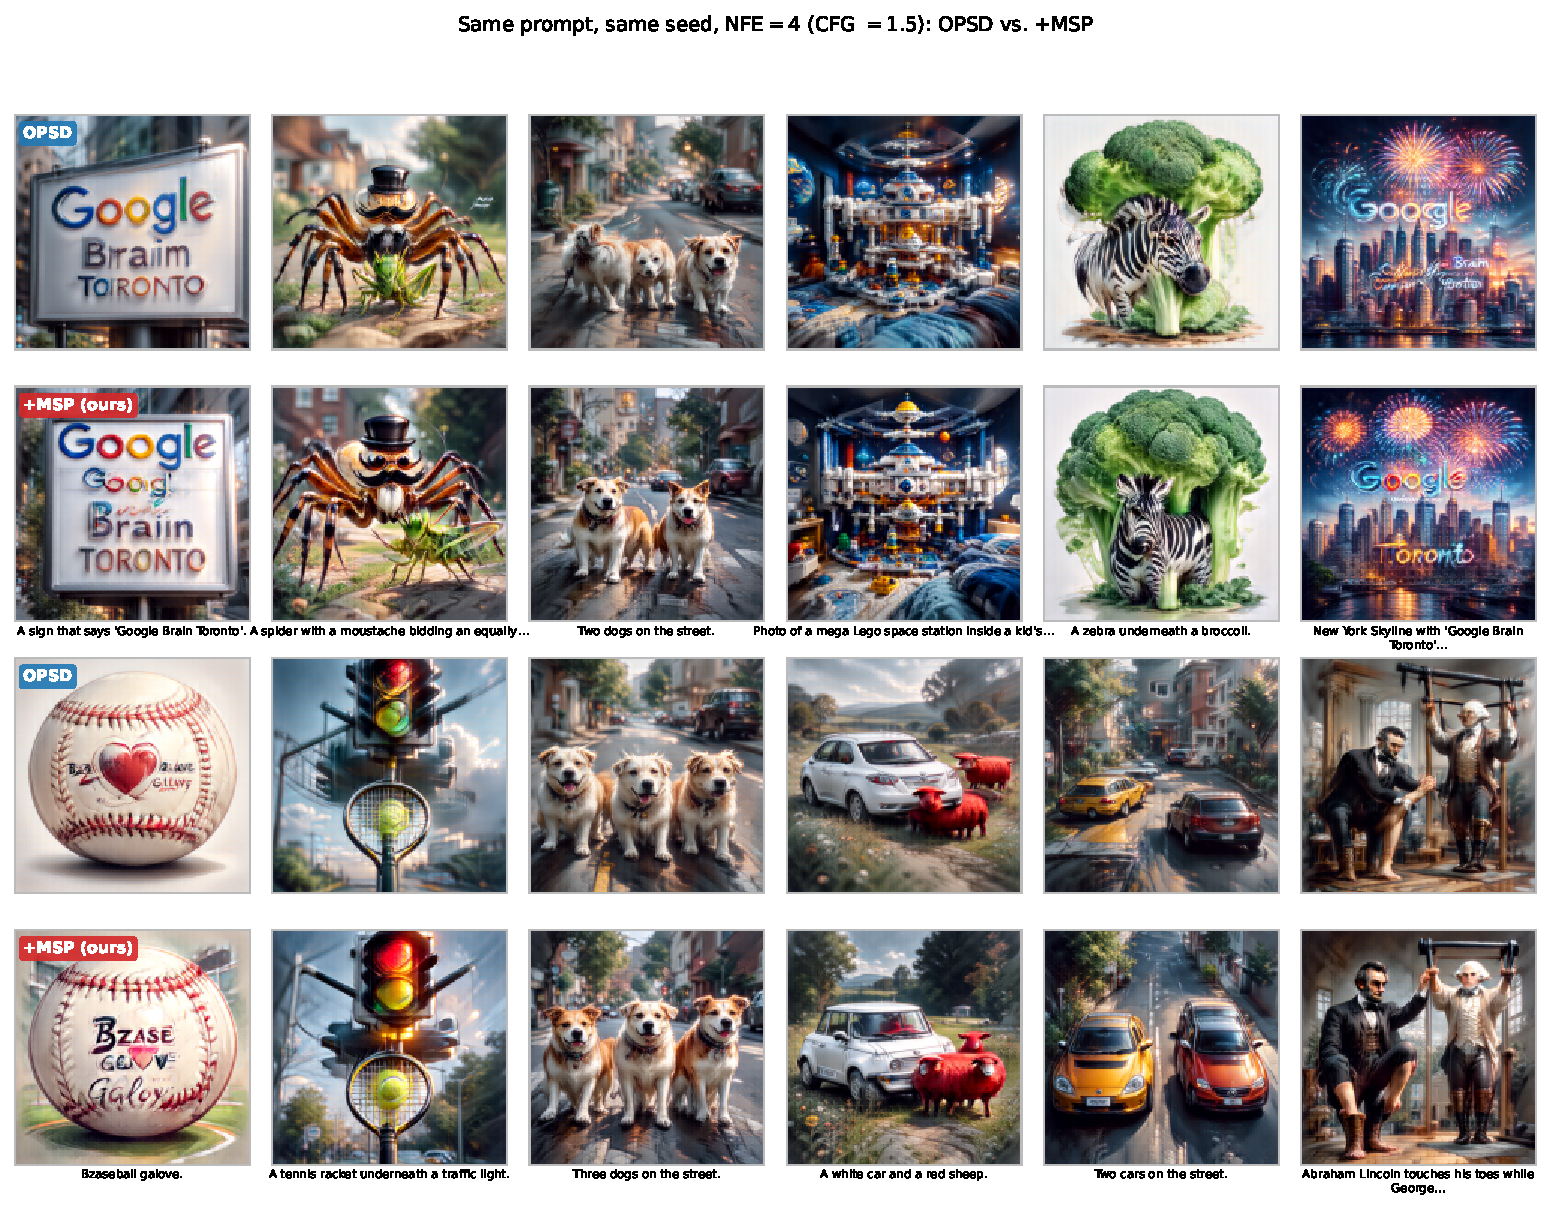
\includegraphics[width=\linewidth]{fig6_qualitative_cfg.pdf}
\caption{\textbf{Four sampling steps, same prompt, same seed; only the model changes.}
\emph{All twelve} prompts selected in advance by a fixed rule (above-median absolute score
under our model, ranked by paired improvement) are shown, with no second pass of manual
filtering; an unselected panel is in App.~\ref{app:qual}. The rule favours prompts whose
differences are checkable by eye rather than by taste: object counts (\emph{two} dogs ---
canonical renders three), spatial relations (the racket \emph{underneath} the traffic
light), and text. Two panels are ties and one (Lincoln) favours canonical; we show them.
These panels are rendered at guidance scale $1.5$ rather than the CFG-free setting used for
every number in this paper, because the CFG-free protocol is a poor \emph{display} setting
at four steps (App.~\ref{app:protocol}); the quantitative protocol is unchanged.}
\label{fig:qual}
\end{figure}

\section{Why moving the query is a trade and propagating is not}
\label{sec:analysis}

\paragraph{A measured exchange rate.} Fix a rollout state $z_k$ and its anchor $y_0^{(k)}$.
Target construction moves $y_0^{(k)}$ a bounded distance and buys some reward. Define the
\emph{exchange rate} at that state as the realized local-reward gain per unit of relative
target displacement, $\widetilde R(\bar y_+)-\widetilde R(y_0)$ divided by
$\|\bar y_+-y_0\|_2/\|y_0\|_2$. Measured on $32$ held-out prompts with the trained
behavior policy, the reward-gradient construction gives
\begin{center}
\begin{tabular}{lcccc}
\toprule
$\sigma$ & $0.278$ & $0.465$ & $0.707$ & $0.913$\\
\midrule
exchange rate & $\mathbf{0.457}$ & $-0.46$ & $0.033$ & $0.0066$\\
\bottomrule
\end{tabular}
\end{center}
The query level chosen by \opsd is the only level where a unit of displacement buys a
substantial \emph{positive} amount: one step higher the construction is actively harmful,
and two or more steps higher it buys an order of magnitude less. \textbf{Moving the query away from it therefore buys trajectory
coverage at the price of target quality.} Propagation does not make that exchange: it
keeps the best construction site and reuses the resulting target elsewhere.

\paragraph{The trade is visible in the training objective itself.} If (A) optimizes a
worse target, it should reach a lower value of the training objective. It does. Over a
full $100$-update run, comparing each arm to its own matched canonical baseline at the
same rollout length,
\begin{center}
\begin{tabular}{lcc}
\toprule
& peak training reward & vs.\ matched canonical\\
\midrule
(A) query $\sigma\!:\,0.278\to0.465$ & $1.5964$ & $\mathbf{-0.0178}$\\
(C) \MSP & $1.6577$ & $\mathbf{+0.0415}$\\
\bottomrule
\end{tabular}
\end{center}
Moving the query lowers the height reached on the training objective; propagating raises
it. (Arms with a shortened rollout are excluded from this comparison because their
training reward is computed on a different sampling schedule and is not comparable. We use
this quantity only as a statement about the training objective, and draw no held-out
conclusion from it.)

\paragraph{Why propagation is not merely a smaller learning rate.} Equation~\eqref{eq:msploss}
divides the main-state term by $1+|\mathcal K|$, so one might suspect that \MSP simply
under-weights the original loss. It does not: halving the learning rate is significantly
\emph{harmful} in this setting ($-8.82$ MDE at $100$ updates), whereas \MSP is positive.
The extra states must therefore contribute useful gradient, and contribute enough to more
than offset the down-weighting of the main term.

\paragraph{Why the gain grows as the budget shrinks.} At $40$ steps both models traverse
every noise level with a small per-step $\Delta\sigma$, and the low-noise portion of the
trajectory can repair mid-noise errors. As the budget falls, each step spans a larger
$\Delta\sigma$ and the mid-noise transitions carry proportionally more of the generation;
this is exactly the region that propagation supervises and that the single-query baseline
never sees a loss at. Consistent with this, the gain is flat between $40$ and $10$ steps --
where neither model degrades -- and rises monotonically below $10$
(Fig.~\ref{fig:curves}).

\section{Conclusion and Limitations}
\label{sec:conclusion}

We asked where the reward target of an on-policy distillation procedure should be applied.
Moving the query state to higher noise -- whether directly or implicitly by shortening the
training rollout -- buys large few-step gains at zero or negative cost, but keeps none of
them at the full budget, where the change turns slightly negative and stops clearing our
threshold; the two routes are the same mechanism and produce the same gain curve.
Propagating one reward-constructed target to several noise levels of the same trajectory
avoids the trade: it is the only one of the three placements that clears the significance
threshold at every sampling budget on both prompt sets, it costs $1.21\times$ in training
time, and it requires no additional reward evaluation. The two are composable, and the
combination is the strongest few-step configuration we measured. One mechanism
therefore covers the whole deployment range: propagation alone when a single model must
serve every budget, propagation with a shortened rollout when few-step inference is the
target.

\paragraph{Limitations.}
\begin{itemize}[leftmargin=1.4em,itemsep=2pt]
\item \textbf{One base model; comparisons at one budget.} All results are on SD3.5-Medium
with LoRA. The reproduction itself is verified at the published $300$-update budget and
matches it on all five evaluators (Sec.~\ref{sec:exp:repro}), but every \emph{comparison}
between propagation and the canonical procedure is made at $100$ updates. We do not know
how the placement effect scales with model size or with a longer schedule.
\item \textbf{The gain has a measured operating range, and we mapped its edges.} Three
separate experiments bound it. (i) \emph{Branch coefficient}: a $2\times2$ on the same joint
objective shows that raising $\beta$ from the published $0.1$ to $1.0$ does not merely
remove the gain but reverses it, from $+10.70$ to $-15.40$ MDE at four steps
(App.~\ref{app:rewardspec}). (ii) \emph{Training length}: at the published $300$ updates the forty-step gain
is gone in both of two independent seeds ($+1.02$ / $+0.24$ MDE in one, $-9.25$ / $-14.28$ in
the other), while at four steps the seeds split: one keeps a significant lead at every
checkpoint ($+8.16$ MDE at $300$), the other peaks near $200$ and ends $7.2$ MDE behind.
Late collapse is therefore a risk we observed once in two runs rather than a ceiling we can
locate (App.~\ref{app:budgetceiling}). (iii) \emph{Objective}: the
reward-specific runs disagree among themselves, spanning a significant loss, two null
results and a significant gain. Propagation as we measure it is
therefore a method for the published joint objective at its published $\beta$, whose
forty-step gain we can claim only for at most a couple of hundred updates -- the setting all our comparisons use, but narrower
than reward distillation in general, and we have not established why the edges fall where
they do.
\item \textbf{On single rewards the sign of the effect depends on the reward.}
Our headline result is on the three-reward objective the published method uses for its main
table. Trained on one reward at a time under the published reward-specific recipe, the
outcome is not uniform: at four steps propagation is \emph{harmful} on PickScore ($t=-15.68$
and $-14.12$ on the two prompt sets), neutral on HPSv2.1 and on CLIPScore, and \emph{helpful}
on ImageReward ($t=+12.11$ and $+7.92$); on all four, as on the joint objective, the effect at
forty steps is null. A fifth recipe, Aesthetic, yields no verdict: both of its arms end below
the untrained base model on the composite while the score they optimise doubles, so there is no
few-step quality there to compare (App.~\ref{app:rewardspec}). We report every one of these
because the comparison was pre-registered, and we draw no pattern from four points. One
reading is ruled out: because the positive case is a single reward, propagation does not
\emph{require} an objective that mixes several rewards. What the reward-specific block does
not isolate is $\beta$, which it also changes from $0.1$ to $1.0$; the $2\times2$ above shows
that change alone, at a fixed three-reward objective, is enough to reverse the sign.
\item \textbf{Held-out significance at the full budget.} On the held-out prompt set,
ImageReward favours \MSP significantly for $\mathrm{NFE}\le10$ but not at $20$ and $40$
($t=+1.50,+1.18$). The full-budget claim rests on the reported composite.
\item \textbf{We do not compare against dedicated few-step distillation.} The comparison
would be informative but is a different experiment; see Sec.~\ref{sec:related}.
\item \textbf{Placement is studied on a fixed schedule family.} We vary which states of a
rectified-flow schedule are used; we do not study continuous or learned placement.
\end{itemize}


\bibliographystyle{plainnat}
\bibliography{refs}

\appendix
\section{Measured noise floor}
\label{app:floor}

Effect sizes in reward alignment are frequently comparable to run-to-run variation, so we
measured the variation rather than assuming it. We evaluated $8$ \emph{unmodified}
canonical arms -- differing only in training hardware (A100/H100/H200), world size ($3$ or
$4$), or random seed -- at the same outer epoch under the identical protocol, and formed
all $28$ pairwise differences of the reported composite.

\begin{center}
\begin{tabular}{lccc}
\toprule
& median $|\Delta|$ & mean $|\Delta|$ & max $|\Delta|$\\
\midrule
$28$ canonical-vs-canonical pairs & $0.39$ MDE & $0.46$ MDE & $1.23$ MDE\\
\bottomrule
\end{tabular}
\end{center}

Among pairs that match on \emph{all} of hardware, world size and seed -- i.e.\ pure
re-runs of the same configuration -- differences range from $0.06$ to $0.56$ MDE, the
latter with a per-image $t$ of $+1.95$. Per-image $t$ is computed over $1000$ images and
is therefore easy to make large; it does not measure run-to-run variation. We consequently
adopt the thresholds stated in Sec.~\ref{sec:exp:protocol}.

We also calibrated the two nuisance axes separately: changing world size from $3$ to $4$
on identical hardware is worth $+0.17$ MDE ($t=+0.58$), and the same canonical
configuration on H200/$4$ versus A100/$3$ differs by $0.07$--$0.54$ MDE across six
(checkpoint, prompt set, budget) cells, with $|t|<1.2$ in five of six. Cross-hardware
comparisons of two \emph{differences} therefore carry at most $\approx0.55$ MDE of slack.

The same arms also bound run-to-run variation on the \emph{absolute} scores, which is what
a reproduction claim rests on. Across seven unmodified canonical runs spanning three GPU
types, two world sizes and two random seeds, the full range of each reported column at
$100$ updates is:

\begin{center}
\begin{tabular}{lccccc}
\toprule
& Pick & CLIP & HPSv2.1 & Aes & ImgR\\
\midrule
median & $24.66$ & $0.316$ & $0.370$ & $5.90$ & $1.43$\\
full range & $0.02$ & $0.002$ & $0.001$ & $0.03$ & $0.02$\\
\bottomrule
\end{tabular}
\end{center}

Training is therefore reproducible at the absolute-score level to well under one part in a
hundred on every column; when we compare an absolute score against a published one, the
binding uncertainty is the evaluation pipeline (Sec.~\ref{sec:exp:repro}), not the training
run.

The headline \emph{difference} is similarly stable across independent training jobs. Our
$300$-update runs pass through $100$ updates on the way, so their checkpoints at that point
give a second, independently trained measurement of the same comparison at the same seed:
$+10.26$ versus $+10.70$ MDE at four steps and $+4.76$ versus $+5.62$ at forty on DrawBench,
differences of $0.44$ and $0.85$ MDE. Both sit inside the canonical-versus-canonical floor
measured above, and the run-to-run spread is \emph{smaller} than the seed-to-seed spread
($1.05$ MDE at four steps), which is the expected ordering.

\section{Held-out evaluator calibration}
\label{app:evalcal}

We required a held-out evaluator that actually tracks the quantity being optimized. Across
$12$ arms spanning $-35$ to $+18$ MDE on the reported composite, measured against a common
canonical baseline:

\begin{center}
\begin{tabular}{lcc}
\toprule
& $r$ with reported composite & sign agreement\\
\midrule
ImageReward & $\mathbf{+0.894}$ & $\mathbf{12/12}$\\
Aesthetic   & $-0.395$ & $4/12$\\
\bottomrule
\end{tabular}
\end{center}

Aesthetic is \emph{anti}-correlated and agrees in sign less often than chance; the most
extreme case is an arm at $-14.19$ MDE on the composite with Aesthetic $t=+27.70$. We
therefore report ImageReward as the held-out evaluator throughout and do not report
Aesthetic. We flag this because Aesthetic is commonly reported in this literature.

\section{Pairing requirements}
\label{app:pairing}

An arm and its baseline must match on training hardware, world size, random seed, and
outer epoch. Two concrete failures we encountered illustrate the need:
comparing an arm at $50$ updates against a baseline at $100$ updates produced a spurious
$-12.32$ MDE that is almost entirely the checkpoint difference; and comparing an arm to a
baseline trained on different hardware inflated a $+17.39$ MDE effect to $+18.34$ MDE.

\section{Sampling schedules and a degenerate query state}
\label{app:schedule}

The $\sigma$ schedules used, obtained from the model's own scheduler:
\begin{center}
\begin{tabular}{ll}
\toprule
$N$ & $\sigma_0,\dots,\sigma_N$\\
\midrule
$10$ & $1.000,\,0.960,\,0.913,\,0.858,\,0.790,\,0.707,\,0.602,\,0.465,\,\mathbf{0.278},\,0.009,\,0$\\
$6$  & $1.000,\,0.923,\,0.819,\,0.668,\,\mathbf{0.432},\,0.009,\,0$\\
$4$  & $1.000,\,0.858,\,\mathbf{0.602},\,0.009,\,0$\\
\bottomrule
\end{tabular}
\end{center}
Because the query is selected by $\argmin_j|\sigma_j-\sigma^\star|$
(Eq.~\eqref{eq:query}), shortening the rollout \emph{implicitly} moves the query: at
$N\!=\!6$ the selected state is $\sigma_q=0.432$.

At $N\!=\!4$ the selection is pathological. Since
$|0.602-0.278|=0.324>|0.009-0.278|=0.269$, the default request selects the near-clean
state $\sigma_q=0.00893$, where $y_0\approx z_q$ and target construction degenerates; the
resulting run peaks at update $15$ and then declines monotonically. A ``train at $4$
steps'' baseline must therefore pin $\sigma^\star$ explicitly to the schedule's
second-to-last non-degenerate state. \textbf{This is itself a finding: a $4$-step rollout
does not contain \opsd's design query state.}

\section{Training cost}
\label{app:cost}

Wall-clock per optimizer epoch over the full $100$-update run, on identical hardware and
world size:
\begin{center}
\begin{tabular}{llcc}
\toprule
hardware & configuration & min/epoch & relative\\
\midrule
\multirow{3}{*}{H200 $\times4$} & canonical & $2.79$ & $1.00\times$\\
 & $+$ \MSP ($|\mathcal K|=2$) & $3.36$ & $\mathbf{1.21\times}$\\
 & $+$ \MSP ($|\mathcal K|=3$) & $3.59$ & $1.28\times$\\
\midrule
\multirow{2}{*}{H100 $\times4$} & canonical & $2.77$ & $1.00\times$\\
 & $+$ \MSP ($|\mathcal K|=2$) & $3.39$ & $\mathbf{1.22\times}$\\
\midrule
H200 $\times4$ & $6$-step rollout & $2.54$ & $0.90\times$\\
\bottomrule
\end{tabular}
\end{center}
Each figure is the median per-epoch wall clock over a run's checkpoint timestamps, dropping
the first twenty epochs so that start-up is excluded. The two-state default costs
$1.21\times$ on H200 and $1.22\times$ on H100, measured on the joint and the reward-specific
objective respectively, so the figure is not specific to one accelerator or one reward. The
marginal cost of a third state is a further $+0.07\times$.

\section{Checkpoint independence}
\label{app:ckpt}

The few-step gain of propagation over canonical at $4$ sampling steps, as a function of
training checkpoint (paired, $n=1000$, MDE units). Every entry compares an arm against a
canonical baseline trained on the \emph{same} hardware and world size at the \emph{same}
checkpoint; cells without such a control are left blank rather than filled with a
cross-hardware comparison.
% 自动生成,勿手改。源:paper_figs/make_table_ckpt.py
\begin{center}
\resizebox{0.98\linewidth}{!}{%
\begin{tabular}{ll ccccc c ccccc}
\toprule
& & \multicolumn{5}{c}{\textbf{NFE}$=$\textbf{4}} & & \multicolumn{5}{c}{\textbf{NFE}$=$\textbf{40}} \\
\cmidrule(lr){3-7}\cmidrule(lr){9-13}
$\mathcal K$ & set & $20$ & $30$ & $50$ & $80$ & $100$ & & $20$ & $30$ & $50$ & $80$ & $100$\\
\midrule
$\mathcal K=\{3,6\}$ (default) & DrawBench & $+6.66$ & $+5.56$ & $+7.52$ & $+10.42$ & $+10.70$ & & $+2.39$ & $+3.44$ & $+3.19$ & $+5.27$ & $+5.62$ \\
 & Unseen-1k & $+5.95$ & $+4.83$ & $+6.06$ & $+8.19$ & $+8.20$ & & $+1.38$ & $+1.50$ & $+1.22$ & $+3.03$ & $+3.34$ \\
\addlinespace[2pt]
$\mathcal K=\{5,6,7\}$ & DrawBench & $+8.16$ & $+5.43$ & $+7.05$ & $+9.15$ & $+8.48$ & & -- & -- & $+1.46$ & -- & $+2.51$ \\
 & Unseen-1k & $+7.37$ & $+5.38$ & $+6.09$ & $+7.62$ & $+6.47$ & & -- & -- & $-0.15$ & -- & $+0.92$ \\
\addlinespace[2pt]
\bottomrule
\end{tabular}}
\end{center}

The dip at $30$ updates appears on \emph{both} prompt sets, so it is a property of the
training trajectory rather than evaluation noise. Every cell exceeds $+5.38$ MDE, so the
effect does not depend on stopping at $100$ updates.

\begin{figure}[h]
\centering
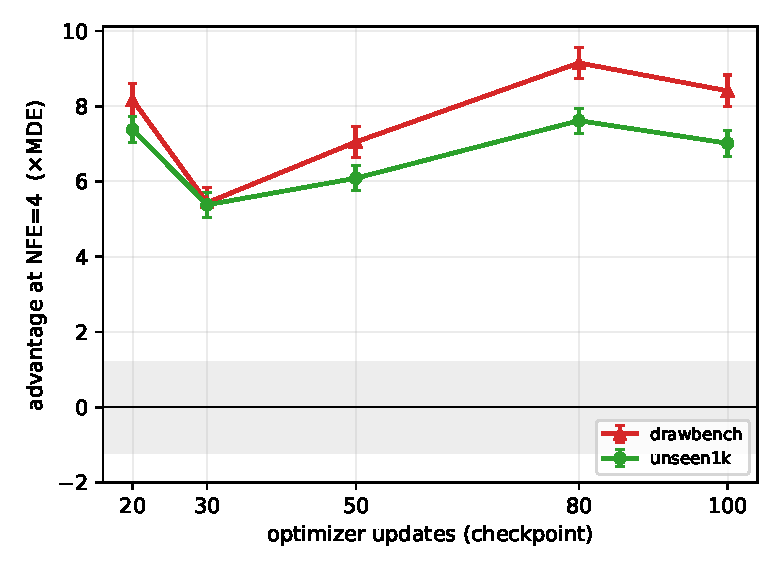
\includegraphics[width=0.78\linewidth]{fig4_advantage_vs_ckpt.pdf}
\caption{Few-step advantage of \MSP over canonical as a function of training checkpoint.
The effect is present from the earliest checkpoint we evaluate and does not depend on
stopping at $100$ updates.}
\label{fig:ckpt}
\end{figure}

\section{Training length: the gain at the published budget}
\label{app:budgetceiling}

Every other result in this paper is measured at $100$ updates. To follow the comparison to
the published $300$ we trained two independent pairs of runs, each pair a propagation run and
a canonical run with the same seed on the same node and world size, and evaluated both members
of a pair at the same five checkpoints. The second pair was pre-registered as a replicate after
the first showed a late collapse.

\begin{figure}[h]
\centering
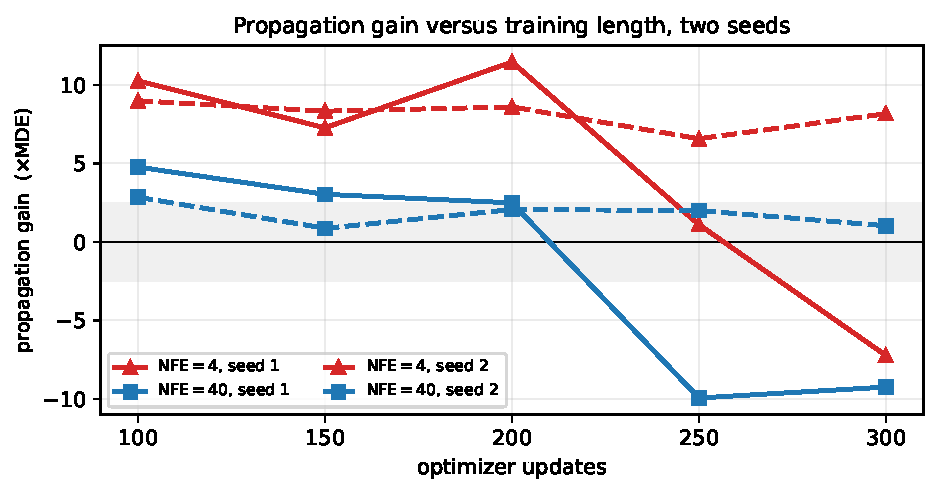
\includegraphics[width=0.74\linewidth]{fig11_gain_vs_updates.pdf}
\caption{\textbf{Propagation gain versus training length}, DrawBench, for two independent
pairs of $300$-update runs (solid: seed 1, dashed: seed 2); each point pairs the two runs of
one seed at the same checkpoint. Shaded: $\pm2.5$ MDE, the band a single seed cannot resolve.
At four steps seed 1 peaks at $200$ updates ($+11.46$) and is $-7.23$ by $300$, while seed 2
stays between $+6.57$ and $+8.99$ at every checkpoint. At forty steps neither seed is above
the band at $300$ updates.}
\label{fig:budgetceiling}
\end{figure}

The two seeds disagree about what happens after $200$ updates and agree about forty steps.
At four steps seed 2 keeps a significant lead at every checkpoint ($+8.99$, $+8.32$, $+8.60$,
$+6.57$ and $+8.16$ MDE on DrawBench, $+3.55$ to $+7.72$ on Unseen-1k, every cell $t\ge8.8$),
whereas seed 1 collapses from $+11.46$ at $200$ updates to $-7.23$ at $300$. At forty steps
the seed-2 gain is small throughout ($+0.86$ to $+2.84$ on DrawBench, $+0.03$ to $+1.71$ on
Unseen-1k) and at $300$ updates is $+1.02$ / $+0.24$ MDE, a tie by our threshold; seed 1 is
$-9.25$ / $-14.28$. So the late collapse is something a run \emph{can} do rather than something
it reliably does --- one run of two --- and neither seed supports a forty-step gain at the
published budget. We report the seeds side by side rather than averaged: at $300$ updates an
average would be dominated by the seed-1 collapse and would describe neither run.

The rest of this section concerns the seed-1 collapse. Two readings are consistent with it and
we cannot separate them. The training reward of the propagation arm peaks higher than the canonical arm's ($1.7051$ versus $1.6626$, both
near epoch $227$) and then falls back to $94.5\%$ of its own peak while the canonical arm
holds $97.8\%$, so the collapse is visible in the training objective as well as in the
evaluation.

Two further measurements bear on which reading is right, and both point away from the
extra states. First, \emph{the collapse does not recur} in the independent seed-2 pair above, nor in a
run that resumes the seed-1 propagation arm from its own $200$-update checkpoint and continues
with propagation still on: over updates $250$ to $300$ that run \emph{gains} $3.80$ MDE at four
steps on DrawBench while the continuous run loses $5.93$. Second, it is not an evaluation artifact: averaging the weights of checkpoints
$280$, $290$ and $300$ leaves the gap to canonical unchanged ($-7.23$ to $-7.45$ MDE at
four steps, and $-11.81$ to $-11.93$ on Unseen-1k), so a single noisy checkpoint is not what
produces it. Taken together the collapse looks like an optimisation-trajectory event rather
than a property of propagating to extra states.

The seed-2 pair is the clean replicate that the resumed arm could not be: resuming by itself
moves the score a great deal in this setting ($+16.11$ MDE at four steps against the continuous
arm at $300$ updates), so on its own the resumed arm could have been masking the collapse rather
than showing it was never there. With both, we read the collapse as a risk rather than a ceiling:
it happened in one of two independent runs, and two runs are too few to estimate how often.

That last perturbation turns out to be informative in its own right, because it is not generic.
Applying the same restart to the \emph{canonical} arm --- resuming it from its own $200$-update
checkpoint and continuing canonically to $300$ --- moves its score by $-0.38$ and $-0.03$ MDE on
DrawBench at four and forty steps and by $-0.06$ and $-0.32$ on Unseen-1k, four cells all inside
the $1$ MDE band we treat as no effect ($|t|\le1.65$). The same perturbation on the propagation
side is $+16.11$ and $+11.56$ on DrawBench and $+19.08$ and $+15.27$ on Unseen-1k. A restart is
therefore not an evaluation perturbation that any run of this kind would respond to; it is
specific to weights trained with propagation. The only discontinuity a resume introduces is that
the live parameters are replaced by their own exponential moving average, since checkpoints are
written from the EMA while the optimiser, EMA buffer and RNG states are all restored --- so what
a restart changes is the point the last $100$ updates start from, not the parameters that get
evaluated. Averaging final parameters after the fact does not reproduce the effect on either
side: souping checkpoints $280$, $290$ and $300$ moves the propagation arm by $-0.49$ to $-1.70$
MDE and the canonical arm by $-0.01$ to $-0.45$ across the same four cells. Why the propagation
arm's live parameters sit somewhere from which a further $100$ updates end up so much worse than
from their own average, we have not measured. What we can say is that the seed-1 collapse is not robust to a perturbation as small as
restarting the same run from its own checkpoint. Whether it is over-optimisation specific to the extra states, or a generic
late-training instability that propagation reaches sooner because it optimises faster, is not
something these runs can decide.

For the seed-1 pair one practical consequence is worth stating plainly. If propagation is stopped at $200$
updates --- two thirds of the published training cost --- it is still $+6.10$ MDE ahead of
the canonical run trained for the full $300$ at four steps, though $-2.63$ behind it at
forty. Spending the remaining third on the canonical objective instead of stopping removes
that forty-step deficit: a run that propagates for $200$ updates and then continues
canonically to $300$ is $+11.44$ / $+9.66$ MDE ahead at four steps and $+5.65$ / $+4.64$ ahead
at forty (DrawBench / Unseen-1k), measured against a canonical run that was itself restarted at
$200$ updates so that the restart discussed above is present on both sides.

We do not read that as a gain from switching objectives. The switch measured on its own ---
against the same restarted propagation run continued with propagation still on --- is $+2.19$
/ $+2.33$ MDE at four steps, below the $2.5$ MDE threshold a single seed has to clear
elsewhere in this paper, and its share of the total fell from $34.1\%$ / $30.4\%$ at $250$
updates to $19.1\%$ / $24.1\%$ at $300$. The larger part of the difference is carried by the
restart effect above, which we do not understand. This is one seed, we did not pre-register an
early-stopping rule, have no held-out split for choosing a checkpoint, and chose the switch
point after seeing where the gain peaked --- so we report the whole of it as an observation
about these runs rather than as a schedule we would recommend.

\section{Which states to propagate to}
\label{app:family}

Our default $\mathcal K=\{3,6\}$ ($\sigma=0.858,\,0.602$) reaches higher noise than the
alternative $\mathcal K=\{5,6,7\}$ ($\sigma=0.707,\,0.602,\,0.465$), which uses \emph{more}
states but tops out at $\sigma=0.707$. At the main checkpoint ($100$ updates) and against
the same control (paired gain in MDE, DrawBench / Unseen-1k):

\begin{center}
\resizebox{0.98\linewidth}{!}{%
\begin{tabular}{lcccccc}
\toprule
$\mathcal K$ & NFE$=2$ & $4$ & $6$ & $10$ & $20$ & $40$\\
\midrule
$\{3,6\}$ (ours) & $+15.3$ / $+16.4$ & $+10.7$ / $+8.2$ & $+7.1$ / $+4.6$ & $+5.8$ / $+3.8$ & $+5.5$ / $+3.4$ & $+5.6$ / $+3.3$\\
$\{5,6,7\}$      & $+20.1$ / $+21.1$ & $+8.5$ / $+6.5$ & $+4.3$ / $+2.7$ & $+2.5$ / $+1.3$ & $+2.0$ / $+0.8$ & $+2.5$ / $+0.9$\\
\bottomrule
\end{tabular}}
\end{center}

One caveat on that table. The $\{5,6,7\}$ arm was trained on a different node type and world
size from everything else here ($3\times$A100 rather than $4\times$H200), so pairing it against
the $4$-GPU control crosses two axes at once. We checked that the conclusion does not depend
on which control we use: against the matched-world-size control instead, its four-step gain is
$+8.04$ / $+6.77$ rather than $+8.48$ / $+6.47$, so the default still leads by $2.2$--$2.7$ MDE
either way. We report the $4$-GPU control in the table because every other row uses it.

Adding a third state does not help, and neither does reaching higher noise. A third
member, $\mathcal K=\{2,3,4\}$ ($\sigma$ up to $0.913$), was trained under the same
protocol. At $100$ updates the default beats it in all four cells -- $-1.30$ and $-1.91$
MDE on DrawBench, $-3.24$ and $-2.63$ on Unseen-1k at $4$ and $40$ steps, the last two
clearing the significance threshold against it. That ordering is not stable across
checkpoints: at $50$ updates the higher set is ahead on DrawBench at four steps
($-1.74$ MDE for the default), so the interior optimum is a statement about the main
checkpoint, not about every point along training. Against the canonical baseline the three
members order as $+10.70/+8.20$ (default), $+9.40/+4.96$ (higher), $+8.48/+6.47$ (lower)
at $4$ steps and $+5.62/+3.34$, $+3.70/+0.70$, $+2.51/+0.92$ at $40$: the default is best
in every cell. The supervision set therefore has an \emph{interior} optimum in the noise
level it reaches, near $\sigma\!\approx\!0.858$.
From $4$ steps upward the two-state set that reaches $\sigma=0.858$ is ahead of the lower
set on both prompt sets, by $+1.7$ to $+3.5$ MDE ($+2.2$ to $+3.5$ on DrawBench, $+1.7$ to
$+2.6$ on the held-out set), and the gap widens with the budget; the lower set decays toward the measured floor while ours flattens at a
positive value (Fig.~\ref{fig:family}). The one exception is $2$ steps, where the lower
set is ahead by about $4.7$ MDE -- at that budget the sampling grid has no interior state
at all ($\sigma\in\{1.000,\,0.009,\,0\}$), so the design principle has nothing to match.

\begin{figure}[h]
\centering
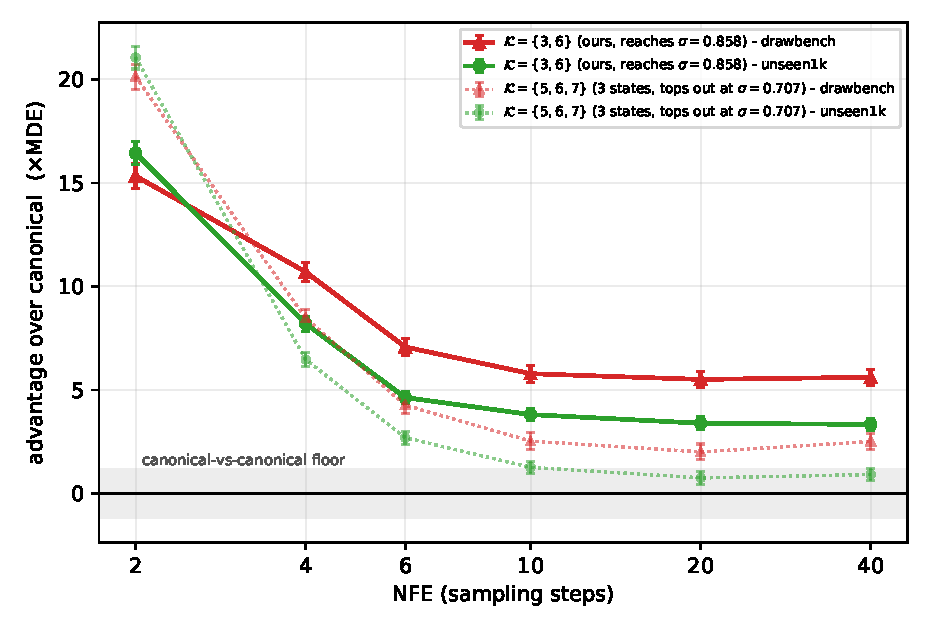
\includegraphics[width=0.78\linewidth]{fig3_advantage_vs_nfe.pdf}
\caption{Advantage over canonical for two members of the propagation family at $100$
updates. Solid: $\mathcal K=\{3,6\}$, which reaches $\sigma=0.858$. Dotted:
$\mathcal K=\{5,6,7\}$, which uses three states but tops out at $\sigma=0.707$. Shaded band
is the measured canonical-versus-canonical floor. The lower set decays toward the floor;
ours flattens at a positive value.}
\label{fig:family}
\end{figure}

\section{Per-axis results}
\label{app:peraxis}

Paired $t$ per reward axis, \MSP versus canonical at $100$ updates:
% 自动生成,勿手改。源:paper_figs/make_table_peraxis.py
\begin{center}
\small
\begin{tabular}{llcccccc}
\toprule
set & axis & NFE$=2$ & $4$ & $6$ & $10$ & $20$ & $40$\\
\midrule
\multirow{4}{*}{DrawBench}
 & PickScore    & $+17.81$ & $+15.71$ & $+12.35$ & $+10.30$ & $+10.80$ & $+11.04$\\
 & CLIP         & $+14.76$ & $+14.32$ & $+10.70$ & $+9.08$ & $+9.22$ & $+9.40$\\
 & HPSv2        & $+34.83$ & $+24.62$ & $+18.48$ & $+14.66$ & $+13.41$ & $+12.89$\\
 & ImageReward  & $+15.14$ & $+11.24$ & $+9.02$ & $+8.32$ & $+7.63$ & $+7.88$\\
\midrule
\multirow{4}{*}{Unseen-1k}
 & PickScore    & $+18.37$ & $+18.09$ & $+11.85$ & $+9.81$ & $+9.66$ & $+10.13$\\
 & CLIP         & $+16.61$ & $+10.01$ & $+7.51$ & $+6.88$ & $+5.99$ & $+5.98$\\
 & HPSv2        & $+40.81$ & $+24.78$ & $+15.98$ & $+10.73$ & $+8.14$ & $+7.42$\\
 & ImageReward  & $+21.50$ & $+9.95$ & $+6.25$ & $+4.35$ & $+1.50$ & $+1.18$\\
\bottomrule
\end{tabular}
\end{center}


\begin{figure}[h]
\centering
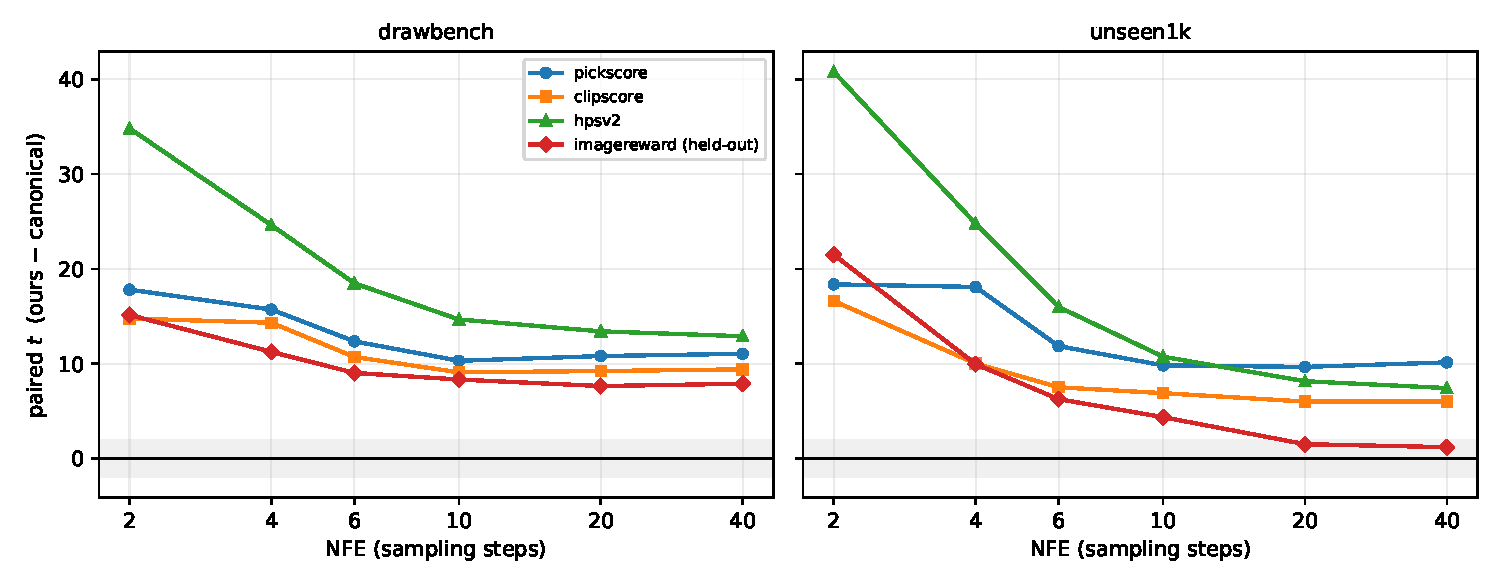
\includegraphics[width=\linewidth]{fig5_peraxis_vs_nfe.pdf}
\caption{Per-axis paired $t$ versus sampling budget. Every axis moves in the same
direction at every budget; the gain is not carried by one reward component.}
\label{fig:peraxis}
\end{figure}

\section{Extreme budget}
\label{app:flow2}

At $2$ sampling steps both models are far outside their usable range -- canonical falls to
a composite of $1.10$, below the \emph{untrained} model at $4$ steps ($1.11$) -- but the
relative ordering is preserved and the gap widens: \MSP is $+15.33$ MDE on DrawBench
($80.2\%$ win rate) and $+16.44$ on Unseen-1k ($84.6\%$). We report this for completeness;
we do not claim $2$-step generation is practical here.

\section{Unselected qualitative samples}
\label{app:qual}

Figure~\ref{fig:qual} selects prompts by a rule fixed in advance: among prompts where our
model's absolute score is above the median, the ones with the largest paired improvement.
For completeness Fig.~\ref{fig:qualunsel} shows a panel drawn without any selection -- the
first eight prompts of the evaluation file in file order.

Those unselected prompts are dominated by DrawBench's adversarial text-rendering and
counting categories. It would be easy to assume that nothing can be seen there because the
model cannot render them; that assumption is wrong. Ranked by paired improvement at four
steps, those same categories are where propagation helps \emph{most}: the twelve
largest-gain prompts are all of this kind, with gains of $+0.18$ to $+0.26$ composite
against a dataset mean of $+0.035$. What makes them poor figure material is their low
\emph{absolute} score, not an absence of difference, which is why the selection rule
conditions on absolute score and then ranks by improvement.

\begin{figure}[h]
\centering
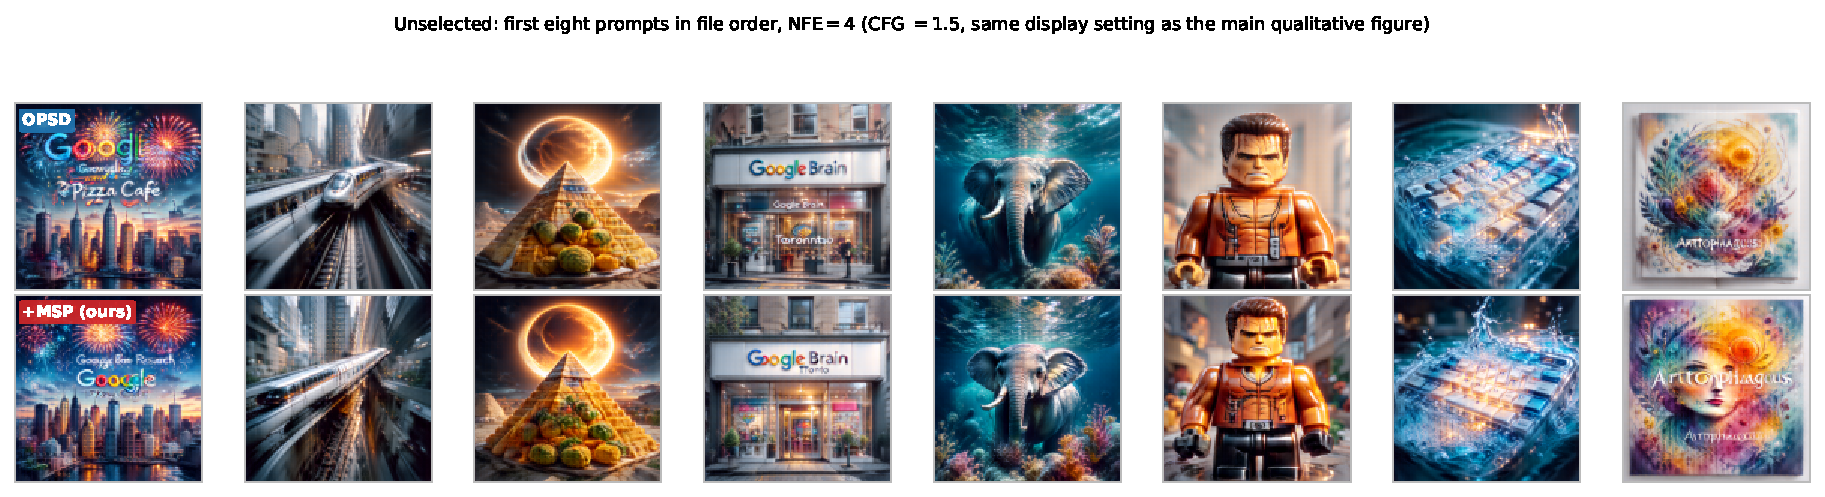
\includegraphics[width=\linewidth]{fig8_qual_unselected.pdf}
\caption{Unselected panel: the first eight evaluation prompts in file order, four sampling
steps, rendered at the same display setting as Fig.~\ref{fig:qual} (guidance $1.5$) so that
the only difference between the two panels is whether the prompts were selected.}
\label{fig:qualunsel}
\end{figure}

\section{The evaluation protocol is not a display protocol}
\label{app:protocol}

Every number in this paper uses the protocol inherited from prior work: $512\times512$,
classifier-free guidance disabled, and the stated number of sampling steps. That protocol
is the right one for \emph{comparison} -- all arms share it and all comparisons are paired
-- but it is a poor setting for \emph{looking at} images, and it also exaggerates one
specific defect.

\paragraph{A frequency measurement.} Reward-trained SD3.5-M checkpoints carry a periodic
texture at the VAE stride ($8$ px) and the patch stride ($16$ px). We quantify it as the
ratio of the spectral magnitude at that period to a local baseline, averaged over the two
image axes; $1.0$ means no periodic structure. The untrained base model scores $1.27$
under the evaluation protocol and $1.03$ once guidance and $40$ steps are restored, so the
structure is not an artifact of the architecture. Reward training raises it: our canonical
reproduction reaches $2.29$ and \MSP $2.57$, while the publicly released single-reward
OPSD checkpoints sit at $1.51$ and $1.56$. Restoring guidance and steps lowers all of them
-- canonical to $1.48$, \MSP to $1.71$, the released checkpoint to $1.22$ -- while the
reported composite \emph{rises} ($1.5460\!\to\!1.6373$ for canonical). The protocol
therefore inflates the defect by roughly $1.5\times$ on top of whatever training produces.

\paragraph{Resolution is not the cause.} At matched guidance and steps, $1024$ and $512$
are indistinguishable ($1.4709$ vs.\ $1.4639$ composite, $1.02$ vs.\ $1.03$ texture).
Removing guidance at $1024$ costs more than halving the resolution does ($1.2380$).

\paragraph{No scalar evaluator sees it.} The texture grows monotonically with training
($1.18$ at $20$ updates to $2.29$ at $100$) while both the reported composite and the
held-out ImageReward improve monotonically over the same range. A frequency measurement is
therefore not redundant with the reward scores; it is the only instrument here that
registers this particular failure.

\paragraph{Choosing a display setting.} Guidance also has an optimum at four steps. Scaling
it from $1.0$ to $4.5$ drives the fraction of pixels clipped to $0$ or $255$ from
$0.4\%$ to $42.8\%$ (canonical) and the composite from $1.5460$ down to $1.3144$. Guidance
$1.5$ maximises the composite ($1.5861$) at $2.6\%$ clipped pixels, and we use it for the
qualitative panels only.

\begin{figure}[h]
\centering
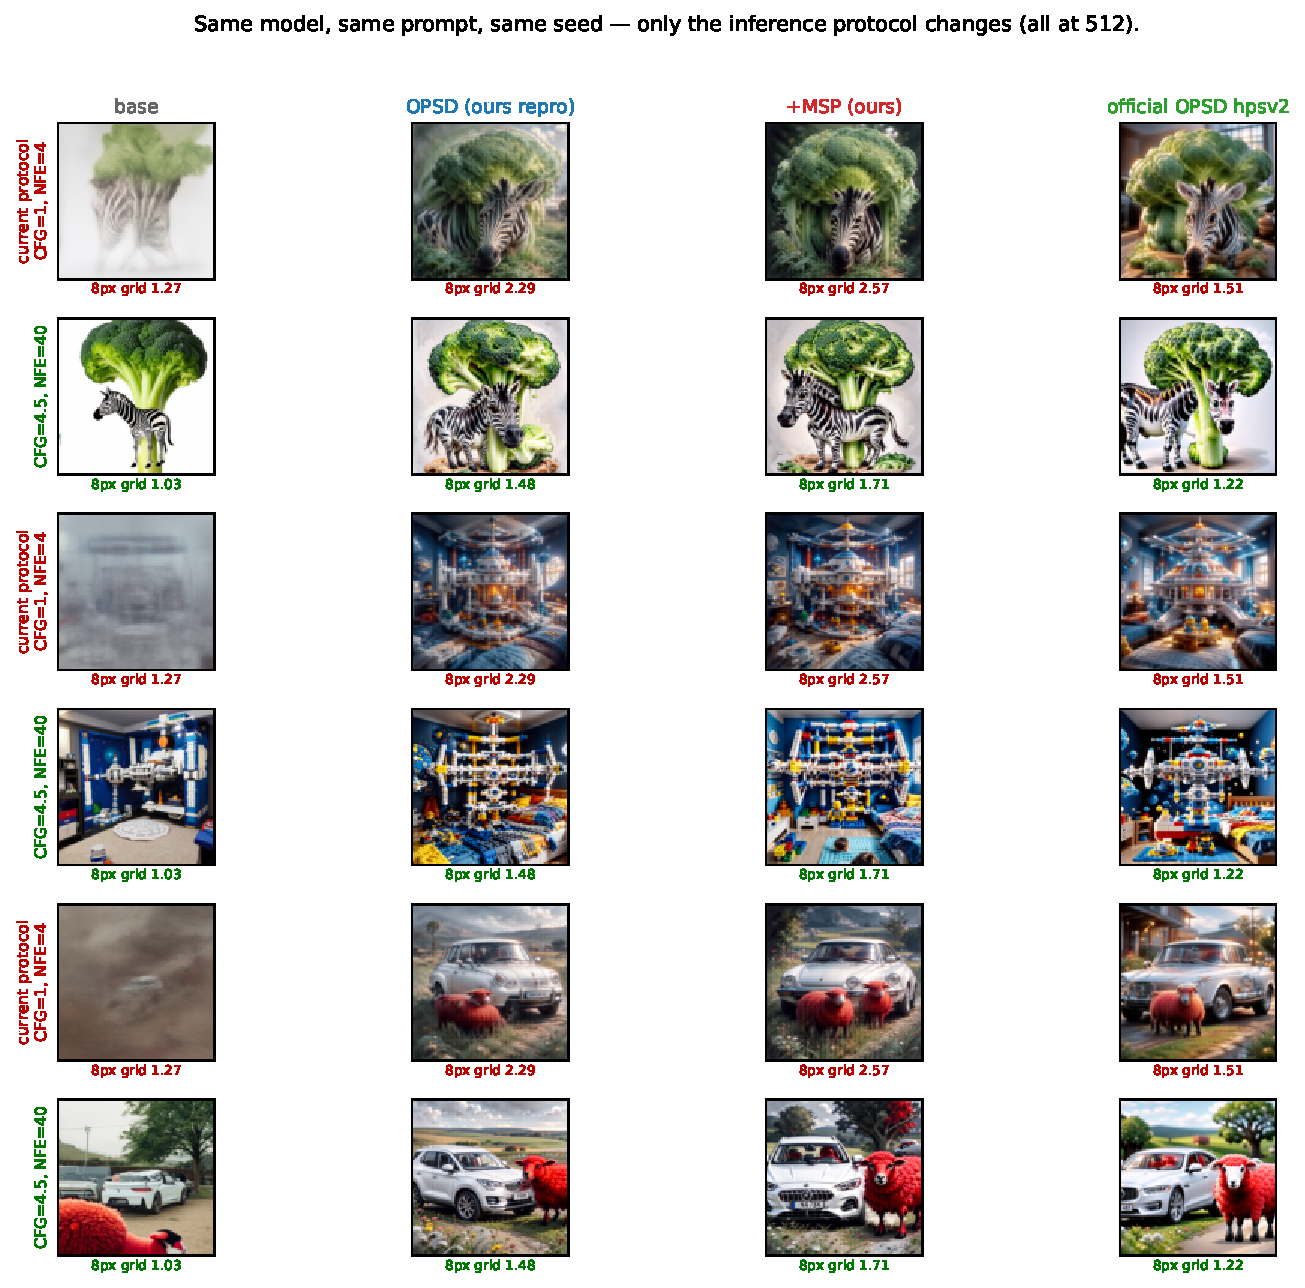
\includegraphics[width=\linewidth]{fig9_protocol_cmp.pdf}
\caption{\textbf{The high-frequency texture is a property of the display protocol, not of
our method.} Same prompts, same seed, $512^2$; only the inference protocol changes between
the two rows of each pair. Numbers are the $8$-pixel (VAE stride) spectral peak divided by
its local baseline; $1.0$ means no periodic structure. Under the evaluation protocol
(CFG-free, four steps) every reward-trained checkpoint is elevated -- including the
\emph{published} \opsd{} checkpoint at $1.51$ -- while the untrained backbone sits at
$1.27$. Raising guidance and the step count brings all four columns down. No scalar
evaluator in this literature detects this; only the spectrum does.}
\label{fig:protocolcmp}
\end{figure}

\section{Does the gain survive on a stronger baseline?}
\label{app:stack}

A method that only helps a weak baseline is fragile. We therefore stack propagation on the
strongest single-arm configuration in our study: a learning-rate variant that reaches
$+17.95$ MDE over canonical at the full budget and $+18.86$ at four steps -- that is, a
baseline whose advantage is essentially flat in the sampling budget (the difference between
the two, $+0.91$ MDE, is the quantity we care about).

Propagating on top of it, at a matched checkpoint, matched hardware and matched seed, and
comparing the two directly rather than through a shared control:

\begin{center}
\begin{tabular}{lcccc}
\toprule
& \multicolumn{2}{c}{\textbf{DrawBench}} & \multicolumn{2}{c}{\textbf{Unseen-1k}}\\
\cmidrule(lr){2-3}\cmidrule(lr){4-5}
& NFE$=4$ & NFE$=40$ & NFE$=4$ & NFE$=40$\\
\midrule
gain over the strong baseline, $50$ updates & $+6.00$ & $+2.40$ & $+4.79$ & $+0.03$\\
gain over the strong baseline, $100$ updates & $+2.95$ & $-3.53$ & $+3.01$ & $-4.68$\\
\bottomrule
\end{tabular}
\end{center}

The budget-dependent part -- the four-step value minus the full-budget value -- is $+3.60$
and $+4.76$ MDE at $50$ updates and $+6.48$ and $+7.70$ at $100$. Propagation on its own
produces $+5.59$ on the same quantity and the learning-rate baseline alone produces
$+0.91$, so the budget-dependence is supplied by the propagation rather than by the
stronger optimisation, and it survives stacking at both checkpoints.

The absolute picture changes between the two checkpoints, and we report it rather than
only the criterion. At $50$ updates stacking is a uniform improvement over the strong
baseline. By $100$ updates it has become a trade: still ahead at four steps, but
$3.5$--$4.7$ MDE behind at the full budget. In this respect the stacked configuration
behaves like the (A$+$C) and (B$+$C) combinations of Sec.~\ref{sec:exp:compose} rather than
like pure propagation, which does not trade.

One caveat: this arm uses the lower supervision set $\mathcal K=\{5,6,7\}$ rather than the
default $\{3,6\}$, because it was launched before the family comparison in
App.~\ref{app:family} settled. The default is better than this member in every cell there,
so the stacking result is a lower bound on what the default would give; we have not run the
default in the stacked configuration and do not report it as if we had.

\section{Reward-specific checkpoints}
\label{app:rewardspec}

The published main table has a second block in which each column is filled by the
checkpoint trained on \emph{that} evaluator, at $100$ optimizer updates and branch
coefficient $\beta=1.0$. We reproduce that block and add propagation to it, under the same
protocol and the same per-reward convention.

% 自动生成,勿手改。源:paper_figs/make_table_rewardspec.py
\begin{center}
\begin{tabular}{l rrr}
\toprule
\textbf{Model} & \textbf{HPSv2.1} & \textbf{Pick} & \textbf{CLIP}\\
\multicolumn{4}{l}{\footnotesize each column is filled by the checkpoint trained on that evaluator}\\
\midrule
SD3.5-M w/o CFG & $0.207$ & $20.59$ & $0.241$\\
$+$ \opsd (reward-specific) & $0.392$ & $24.96$ & $0.320$\\
$+$ \MSP (reward-specific) & $0.391$ & $24.95$ & $0.319$\\
\bottomrule
\end{tabular}
\end{center}


For reference, the published reward-specific row reports HPSv2.1 $0.390$, PickScore
$24.94$ and CLIPScore $0.340$. Cells that are not yet filled are left blank; no number is
borrowed across rewards.

\paragraph{Reproduction.}
Our reward-specific canonical run reaches HPSv2.1 $0.392$ against the published $0.390$ --
a $0.5\%$ agreement, obtained with no tuning beyond matching the stated protocol. Together
with the joint-objective parity of Sec.~\ref{sec:exp:repro} this establishes that the
baseline we improve upon is the published method, not a weakened variant of it.

\paragraph{Every reward-specific run, on the same thresholds.}
Each row compares propagation against the canonical run trained on the \emph{same} single
reward, scored on that reward, at the published $100$-update budget. The verdict column
applies the thresholds fixed in advance (Sec.~\ref{sec:exp:protocol}): $+$ significant gain,
$0$ no effect, $-$ significant loss. The deficit ratio is each model's own four-step deficit
for \MSP divided by the canonical one, as in the table above.

% 自动生成,勿手改。源:paper_figs/make_table_rsverdict.py
\begin{center}
\begin{tabular}{lcccccc}
\toprule
& \multicolumn{2}{c}{NFE$=4$ (paired $t$)} & \multicolumn{2}{c}{NFE$=40$} & &\\
\cmidrule(lr){2-3}\cmidrule(lr){4-5}
\textbf{training reward} & DrawB. & Uns.-1k & DrawB. & Uns.-1k & deficit ratio & verdict\\
\midrule
HPSv2.1 & $+0.27$ & $-0.31$ & $-1.22$ & $-3.67$ & $0.97$\,/\,$0.95$ & $0$\\
PickScore & $-15.68$ & $-14.12$ & $-0.42$ & $-3.09$ & $1.70$\,/\,$1.58$ & $-$\\
CLIPScore & $+5.15$ & $+4.80$ & $-2.30$ & $-2.59$ & $0.48$\,/\,$0.46$ & $0$\\
ImageReward & $+12.11$ & $+7.92$ & $+4.41$ & $+3.52$ & $0.35$\,/\,$0.47$ & +\\
Aesthetic & $-274.71$ & $-292.47$ & $-140.82$ & $-158.02$ & $3.81$\,/\,$4.19$ & n/a$^{\dagger}$\\
\bottomrule
\end{tabular}
\\[2pt]{\footnotesize $^{\dagger}$No verdict: both arms of this pair score \emph{below the untrained}
base model on the reported composite in all four cells, so the comparison is between two
collapsed models and does not measure few-step quality. Numbers are shown unchanged.}
\end{center}


The objectives do not agree with each other --- the four that yield a verdict span a
significant loss, two null results and a significant gain --- which is why the
pre-registration fixed that all of them be reported rather than summarised into one
number.

\paragraph{The reward-specific outcome depends on the reward.}
Propagation is harmful at four steps on PickScore, neutral on HPSv2.1 and on CLIPScore, and
helpful on ImageReward. The fifth recipe, Aesthetic, yields no verdict, for a reason that is
about the recipe and not about propagation: \emph{both} arms end up below the untrained base
model on the reported composite in all four cells ($0.93$--$1.00$ against $1.07$--$1.24$) while
the Aesthetic score they are trained on more than doubles ($4.7$--$5.6$ to $10.2$--$12.2$), and
the gap to the base model widens with further training. Comparing two collapsed models on the
score they are both exploiting does not measure few-step quality, so we report the numbers and
withhold the verdict. On that score propagation is far behind ($t=-46$ at four steps); we state
it rather than omit it, but it is not evidence about the method.

This is a property of the published recipe, not of our run, and the reproduction is what shows
it. The published reward-specific Aesthetic figure is $12.08$ (and $12.09$ for ReFL, $9.11$ for
DiffusionNFT, against $5.12$ for the untrained backbone), and our canonical Aesthetic run
reaches $12.18$ --- a $0.87\%$ difference, inside the $1.6\%$ tolerance of
App.~\ref{app:protocol}. That same checkpoint sits below the untrained backbone on
\emph{all five} other evaluators: composite $0.943$ vs.\ $1.240$, ImageReward $-1.58$ vs.\
$-0.55$, PickScore $17.81$ vs.\ $20.59$, CLIPScore $0.068$ vs.\ $0.241$, HPSv2.1 $0.189$ vs.\
$0.207$. We reproduce the published number closely and report what it costs; we draw no
comparison of methods from it.

There is a second reason this pair is not a comparison, and it is about our run rather than the
recipe: the \MSP arm \emph{diverged}. Its training reward rises normally to $10.34$ at update
$42$, then falls to $4.90$ by update $56$ --- below the $5.75$ it started from, for seven
consecutive updates --- and recovers only to $7.09$ by update $100$, never regaining the peak.
The canonical arm rises over the same range with no comparable event: it never falls below
its own starting value, and its largest drawdown from its running peak is small enough that the
same check does not flag it. At update $100$ the \MSP arm scores
$4.42$ on the objective it was trained to maximise, below the $4.73$ of the untrained backbone.
We state this plainly: propagation was unstable under this recipe. We do not call it a
mechanistic failure of the method, because the instability occurs inside a regime where
\emph{both} arms are worse than no training at all, and we cannot separate ``propagation is
unstable on this objective'' from ``this objective is not trainable''. None of the four
reward-specific pairs that do yield verdicts triggers the same divergence check. This is a second and
independent reason to set Aesthetic aside: App.~\ref{app:evalcal} already shows it is a poor
\emph{yardstick} (anti-correlated with the composite), and this shows it is a poor
\emph{objective}. At the main checkpoint, paired over
$n=1000$ images, on each run's own training reward:

\begin{center}
\begin{tabular}{llccc}
\toprule
prompt set & NFE & \MSP & canonical & paired $t$\\
\midrule
\multirow{2}{*}{DrawBench} & $4$  & $0.3727$ & $0.3725$ & $+0.27$\\
                           & $40$ & $0.3915$ & $0.3920$ & $-1.22$\\
\midrule
\multirow{2}{*}{Unseen-1k} & $4$  & $0.4020$ & $0.4021$ & $-0.31$\\
                           & $40$ & $0.4211$ & $0.4223$ & $-3.67$\\
\bottomrule
\end{tabular}
\end{center}

At the budget where propagation delivers its largest joint-objective gain -- $4$ steps --
the two HPSv2 runs are indistinguishable on both prompt sets ($|t|<0.4$, win rate
$50$--$52\%$). Expressed against the canonical few-step deficit that propagation is designed
to close ($0.0195$ and $0.0201$ HPSv2.1 on the two sets), the change is $+0.7\%$ and
$-0.7\%$: zero to the precision of the measurement.

PickScore is worse than neutral. Trained on PickScore alone, propagation loses $0.58$ and
$0.51$ PickScore at four steps ($t=-15.68$ and $-14.12$, win rates $36\%$ and $38\%$) while
matching the canonical run at forty ($t=-0.42$ and $-3.09$); held-out ImageReward moves the
same way at four steps ($t=-7.57$ and $-3.89$), so this is not an artifact of the PickScore
evaluator. The signature is the inverse of the joint-objective one: measured against itself,
the canonical PickScore run has a four-step deficit of $0.82$ and $0.78$, and propagation
\emph{widens} it to $1.39$ and $1.23$ -- where on the joint objective the same intervention
narrows the deficit from $19.1$ to $13.7$ MDE. The two arms are matched on training
hardware, world size, seed, node and checkpoint, and propagation reaches a \emph{higher}
training reward at every epoch ($0.9381$ versus $0.9320$ at peak), so the loss is not an
optimization failure: the extra states move this objective somewhere that does not survive
a shortened sampler. We pre-registered this comparison, including its
thresholds, before the checkpoints existed, and report it under those thresholds. The
pre-registration also fixed what to do if the reward-specific runs disagree with each
other: report all of them rather than choose, which is what we do above. On CLIPScore the
four-step comparison is positive but short of the threshold ($t=+5.15$ and $+4.80$ against a
pre-registered $5.5$), so it is recorded as no effect; the held-out ImageReward on those same
checkpoints is strongly positive ($t=+9.53$ and $+11.90$), but the pre-registration fixed
held-out as reported-not-decisive for these runs, because their training objective does not
contain it.

The cleanest way to see the scope is one dimensionless number per objective: each model's
own four-step deficit (its $40$-step score minus its $4$-step score), for \MSP divided by
the same quantity for the canonical run. Below $1$ means propagation narrowed the deficit,
above $1$ means it widened it, and the ratio is comparable across objectives that are
measured on different scales.

% 自动生成,勿手改。源:paper_figs/make_table_deficit.py
\begin{center}
\begin{tabular}{lcc}
\toprule
& \multicolumn{2}{c}{\textbf{four-step deficit, \MSP $/$ canonical}}\\
\cmidrule(lr){2-3}
\textbf{training objective} & DrawBench & Unseen-1k\\
\midrule
\textbf{joint three-reward objective} & $0.73$ & $0.72$\\
reward-specific, HPSv2.1 & $0.97$ & $0.95$\\
reward-specific, PickScore & $1.70$ & $1.58$\\
reward-specific, CLIPScore & $0.48$ & $0.46$\\
reward-specific, ImageReward & $0.35$ & $0.47$\\
\bottomrule
\end{tabular}
\end{center}


On the objective the method was developed for, propagation removes about a quarter of the
four-step deficit on both prompt sets. Trained on HPSv2 alone it leaves the deficit where it
was, and trained on PickScore alone it makes it roughly $60$--$70\%$ larger. Whatever makes
propagation work is therefore not present when the target direction is built from a single
reward.

One measurement caveat applies symmetrically to both results: each is a single checkpoint.
At half the budget the sign of the four-step comparison is the opposite of what it is at the
registered checkpoint for \emph{both} completed rewards (HPSv2 $-11.32\to+0.27$, PickScore
$+4.92\to-15.68$), which is why the comparison point was fixed in advance. On the joint
objective the same difference is positive at all five checkpoints we measure.

\paragraph{The two published blocks differ in $\beta$, not only in reward count.}
The protocol that defines these two blocks sets the branch coefficient to $\beta=0.1$ for
the joint objective and $\beta=1.0$ for each reward-specific run. The reward-specific
setting therefore differs from the joint setting in \emph{two} respects at once, and the
neutrality above cannot by itself be attributed to the number of rewards. Because $\beta$
scales the separation between the two branches -- and hence how far the model must move
from its anchor to reach the target -- it is the more direct candidate: where the required
displacement is small, a single query state already supplies it and additional states carry
no new information.

We tested this directly rather than arguing it, by completing a $2\times2$ over
$\beta\in\{0.1,1.0\}$ and $\{$canonical, \MSP$\}$ on the \emph{same} joint objective, which
removes the reward-count difference. All four cells were trained at $100$ updates on one
node, same seed, same world size; the comparison was registered before the fourth cell
existed.

\begin{center}
\begin{tabular}{lcccc}
\toprule
effect of propagation & \multicolumn{2}{c}{DrawBench} & \multicolumn{2}{c}{Unseen-1k}\\
\cmidrule(lr){2-3}\cmidrule(lr){4-5}
 & NFE$=4$ & $40$ & NFE$=4$ & $40$\\
\midrule
at $\beta=0.1$ (published) & $+10.70$ & $+5.62$ & $+8.20$ & $+3.34$\\
at $\beta=1.0$             & $-15.40$ & $-3.11$ & $-9.84$ & $-2.82$\\
\midrule
interaction                & $\mathbf{+26.1}$ & $+8.7$ & $\mathbf{+18.0}$ & $+6.2$\\
\bottomrule
\end{tabular}
\end{center}

The outcome is stronger than the hypothesis predicted. Raising $\beta$ does not merely
remove propagation's benefit -- it \emph{reverses the sign}, from $+10.70$ to $-15.40$ MDE
at four steps, consistently on both prompt sets. Propagation at $\beta=1.0$ also ends far
below propagation at $\beta=0.1$ in absolute terms ($-31.2$ and $-23.5$ MDE at four steps),
so this is not an artifact of the $\beta=1.0$ baseline being weaker; the branch coefficient
limits what propagation can reach, not just where it starts.

A third canonical run at $\beta=0.3$, on the same node and seed, locates the baseline's own
$\beta$ dependence: it loses $0.76$--$1.15$ MDE relative to $\beta=0.1$ across the four cells,
against $5.09$--$6.09$ MDE at $\beta=1.0$. That is $63$--$86\%$ of a straight line through the
two endpoints, so the canonical level degrades roughly linearly in $\beta$ rather than falling
off a cliff. The loss is of the same order at both budgets --- $0.76$--$0.86$ MDE at four steps
against $0.86$--$1.15$ at forty --- so unlike propagation it is not concentrated at few steps. Propagation's effect
swings by $26.1$ MDE over the same interval --- an order of magnitude more than the baseline
moves, and unlike the baseline it is concentrated at few steps. We did not train \MSP at
$\beta=0.3$, so where the sign crosses is not measured; the interaction is large enough that
the gain curve has no reason to follow the level curve.

This settles the question we posed and raises the bar on the explanation. $\beta$ clearly
moderates propagation on the joint objective. But it cannot be the whole story, because the
three reward-specific runs were all trained at $\beta=1.0$ and still disagree with each
other --- neutral, neutral and harmful. We therefore report two facts side by side rather
than one mechanism: the branch coefficient governs whether propagation helps on the joint
objective, and something reward-dependent that we have not isolated governs the outcome
within the reward-specific setting.


\end{document}
